\documentclass[sigconf]{acmart}
\settopmatter{printfolios=true}
%%
%% \BibTeX command to typeset BibTeX logo in the docs
\AtBeginDocument{%
  \providecommand\BibTeX{{%
    Bib\TeX}}}

\setcopyright{acmlicensed}
\copyrightyear{2026}
\acmYear{2026}
\acmDOI{XXXXXXX.XXXXXXX}
\acmConference[RTKS Project]{Real-Time Kernels and Systems Course Project}{July, 2026}{Padua, Italy}

%%
%%  Uncomment \acmBooktitle if the title of the proceedings is different
%%  from ``Proceedings of ...''!
%%
%%\acmBooktitle{Woodstock '18: ACM Symposium on Neural Gaze Detection,
%%  June 03--05, 2018, Woodstock, NY}
\acmISBN{978-1-4503-XXXX-X/2018/06}

\usepackage{enumitem}

\begin{document}


\title{Analysis of "An Empirical Study of Performance Interference: 
Timing Violation Patterns and Impacts"}


\author{Lorenzo Albertin}
\email{lorenzo.albertin@studenti.unipd.it}
\affiliation{%
  \institution{University of Padua}
  \city{Padua}
  \state{Italy}
  \country{IT}
}

\author{Andrea Santi}
\email{andrea.santi.5@studenti.unipd.it}
\affiliation{%
  \institution{University of Padua}
  \city{Padua}
  \state{Italy}
  \country{IT}
}

\author{Caterina Vallotto}
\email{caterina.vallotto@studenti.unipd.it}
\affiliation{%
  \institution{University of Padua}
  \city{Padua}
  \state{Italy}
  \country{IT}
}

\renewcommand{\shortauthors}{Lorenzo Albertin, Andrea Santi, Caterina Vallotto}

\begin{abstract}
This report presents a small-scale experimental analysis of the paper \textit{"An Empirical Study of Performance Interference: Timing Violation Patterns and Impacts"}, which investigates how hardware-induced performance interference can propagate through Cyber-Physical Systems (CPS) and ultimately degrade physical control behaviour. Rather than reproducing the complete TimeTrap framework, we focus on experimentally evaluating selected timing-violation mechanisms and their qualitative effects in controlled virtualized environments.

\noindent The study is organized into two case studies. The first investigates ArduPilot Copter-4.0 running in a Software-in-the-Loop (SITL) environment, where we compare the effects of indiscriminate resource saturation, explicit software delay injection, and a low-priority cache-contention workload after separating sensor emulation from the control thread. The second analyzes the ROS Navigation Stack for TurtleBot3 in Gazebo by injecting controlled delays at different stages of the navigation pipeline, including localization, TF publication, costmap generation, and local planning.

\noindent For both case studies, we define repeatable experimental configurations, introduce custom instrumentation to collect timing and control metrics, and evaluate how timing perturbations affect temporal displacement, data freshness, control-loop execution, navigation behaviour, and mission-level performance. Our results show that explicit software delay injection consistently produces measurable temporal displacement and significant control degradation, while the selected resource-contention workloads do not reproduce the same effects under the adopted virtualized setup. Even though our experiments do not constitute a complete validation of the TimeTrap framework, they qualitatively confirm several of the timing-propagation mechanisms discussed in the original work while highlighting the limitations imposed by virtualization, simulation, and the manual selection of injection points.
\end{abstract}



\maketitle

\section{Problem statement}
The sections ~\ref{sec:1.1} and ~\ref{sec:1.2} are primarily based on the original TimeTrap paper~\cite{li2024timetrap} and on the lecture notes provided during the Real-Time Kernels and Systems course~\cite{T01},~\cite{T01-dep},~\cite{T06},~\cite{T09},~\cite{T11},~\cite{T14}.
\subsection{Scope of the original work}

\textbf{Introduction to Cyber-Physical Systems (CPS)} \label{sec:1.1} \\
%% T01, Paper in generale
The original work "\textit{An Empirical Study of Performance Interference: Timing Violation Patterns and Impacts}" investigates the use of multi-core platforms in modern Cyber-Physical Systems (CPS) and the safety risks of physical control deviations caused by timing constraint violations. To fully understand the operational context of these systems, we have to take into account the fundamental principles of Cybernetics. A CPS interacts continuously with the physical environment through a strict feedback control loop composed of three continuous phases: \textit{sensing} the external environment, \textit{computing} the required correction, and \textit{actuating} the physical response to reach a system goal.
\\
%% T01, T01-approfondimento, Paper in generale
In the domain of Cyber-Physical Systems and real-time embedded systems, temporal predictability and system dependability are crucial. According to dependability theory, it is essential to distinguish between two of its primary attributes:
\begin{itemize}
    \item \textit{Reliability}, which corresponds to the continuity of correct service delivery:
    \item \textit{Safety}, which corresponds to the non-occurrence of catastrophic consequences.
\end{itemize}  
For a Cyber-Physical System, operational correctness is not determined solely by the result of computation; rather, it also strictly depends on the output's timing, meaning that correctness is evaluated in both the time and value domains. Producing a correct value later than its deadline acts as a fault that degrades the feedback control loop, causing an interruption in the continuity of the expected service (which constitutes a  \textit{reliability issue}). Because a CPS continuously interacts with the physical world, this timing-related reliability failure inevitably translates into a physical deviation (e.g. causing a drone to crash or a robot to deviate from its path), compromising the safety of the physical environment.
\\
%% Paper INTRODUCTION (I) SWaP, Paper (II) Orb Slam
Modern autonomous applications can involve complex software pipelines (e.g. environment perception, localization, and motion planning), which demand huge computational power. To satisfy these requirements while keeping Size, Weight, and Power (SWaP) under strict limits, the embedded industry has heavily migrated to multi-core architectures.
\\
\textbf{Multi-core architectures: Contention for shared resources and performance interference} \\
%% T11, T01, Paper 
Multi-core processors are tightly coupled systems where different cores share physical and logical resources, such as the memory bus, memory controllers, and L2/L3 caches. While this architectural shift successfully scales up average computational throughput, it invalidates the premise that an executing task has exclusive control over the physical hardware. Instead, executing tasks continuously contend for shared architectural resources, destroying the timing determinism of single-core architectures. Because these shared hardware components are primarily designed to optimize average-case performance, they can operate adversarially to the predictability needs of a Real-Time System.
\\
%% Paper INTRODUCTION (I) and Abstract, T11, T05
In the context of Real-Time Systems, this hardware-level access contention generates severe performance interference. 
For example, consider how cache coherence mechanisms are affected in multi-core processors. While individual cores rely on private caches (L1) to minimize memory access latency, tasks running concurrently on different cores often access shared memory locations. This concurrent access can cause local cache contents to diverge, risking the use of obsolete data.
Simultaneous requests to use implicitly shared resources necessitate strict access arbitration. Because of this arbitration, running jobs may hold the CPU without making any actual computational progress; this is called \textit{stalling}. This hidden wait time artificially inflates the \textit{Worst-Case Execution Time (WCET)} of the tasks, demonstrating a critical failure of multi-core environments: the WCET is no longer composable. When applying \textit{Response Time Analysis}, where $R_i = C_i + B_i + I_i$, this hardware interference acts as an unpredictable inflation of the execution time ($C_i$) or as invisible interference ($I_i$), which completely compromises the temporal predictability of the system.
\\
%% Notion (T06)
This hardware-level unpredictability is intensified by how modern real-time software is implemented. To program a real-time system correctly, there must be strict alignment between the programmer's intent (what the system needs to do) and the system rules (the temporal constraints that must be met). However, many programming languages lack native timing semantics, making it difficult to enforce these rules effectively. When developers fail to manage these temporal constraints, hardware-induced delays are allowed to propagate through the software layer.
\\
%% Paper, T09
With a deep analysis of real-world CPS software, the authors of the paper identify that this delay propagation leads to severe \textbf{timing issues} in Cyber-Physical Systems. While similar to conventional concurrency bugs (like data races), these timing issues do not necessarily crash the software; instead, they alter algorithm-level semantics and degrade physical control performance. Through these studies, the authors identify three main vulnerabilities that cause timing issues:
\begin{itemize}[nosep]
    \item \textbf{Type I}: Missing timing constraints. The programmer assumes the timing will be predictable and there is no formal rule in the code to guarantee it;
    \item \textbf{Type II}: Incomplete timing constraints. Timing delays are allowed, but the maximum limits are poorly defined;
    \item \textbf{Type III}: Poorly implemented timing constraints. This is often caused by errors in the system's schedulers or bad coordination between tasks.
\end{itemize}
The combination of multi-core hardware interference and these software vulnerabilities results in \textbf{temporal displacement}. This occurs when critical data becomes misaligned in time, causing the CPS to consume stale or desynchronized data, which can trigger catastrophic failures in the physical world.
\\
%% Paper, T09, T01-approfondimento
\textbf{Mechanism: Temporal Displacement}\\
The paper formulates the potential physical impact of this performance interference through the concept of temporal displacement, which represents the difference between the actual timing of the data update and its expected timing. 
From the perspective of Dependability theory, the progression from hardware interference to physical deviation shows the \textit{Fault → Error → Failure} chain. The targeted performance interference injected into the shared hardware acts as a \textit{fault}. This fault alters the timing behaviour, generating a temporal displacement, which constitutes an anomalous internal system state (\textit{error}). The error manifests in the system's external behaviour as a physical deviation (\textit{failure}).
\begin{figure}[t]
    \centering
    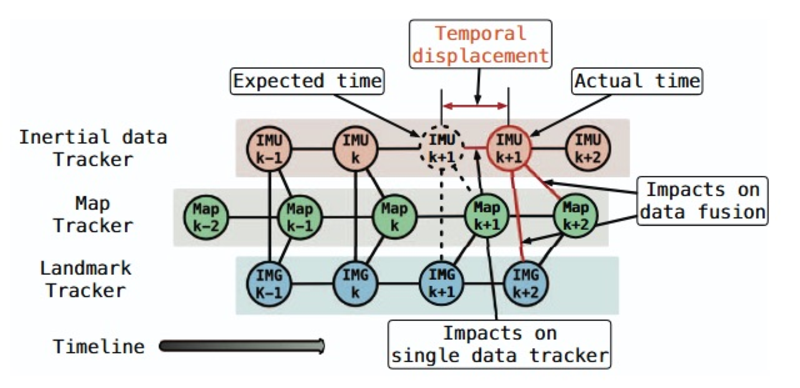
\includegraphics[width=0.80\columnwidth]
        {figures/sensordatatracker.pdf}
    \caption{Temporal displacement. Reproduced from~\cite{li2024timetrap}.}
    \label{fig:sensor}
\end{figure} \\
In modern CPS platforms, tasks do not operate independently; they are organized into processing pipelines, each structured as a transaction that includes a sequence of interdependent tasks. Injecting a delay in a single node, such as a \textit{sensor data tracker} (see Figure~\ref{fig:sensor}), results in a cascading delay that propagates across the entire data flow, causing the error to reach the physical actuators. From the perspective of \textit{End-to-End Analysis}, which evaluates the total timing behaviour across the entire execution pipeline, this dynamic reflects a \textit{producer-consumer dependency} controlled by precedence constraints. A temporal displacement in a producer task introduces a release jitter into the following consumer tasks, such as motion planning or actuation.
This cascading effect desynchronizes the data flow, causing algorithms to evaluate the environment using temporally misaligned data, a condition the authors define as \textit{data misuse}. Ultimately, this dynamic violates the end-to-end deadline, that is the maximum acceptable latency for the entire sensor-to-actuator transaction to complete, and severely degrades the quality of the system's physical response.
\\
It is exactly this vulnerability in the feedback control loop that the authors aim to exploit. While Cyber-Physical Systems typically rely on fail-safe mechanisms to detect severe anomalies and transition the system into a predefined safe operating state, the authors show that targeted timing interference can bypass these mechanisms and cause severe physical deviations in real-world autonomous systems.

\subsection{Purpose of the original work} \label{sec:1.2}
\textbf{Background Literature} \\
% Paper, T01-approfondimento, T14
As explained in the previous section, performance interference in Cyber-Physical Systems is a multi-level issue: it begins with shared hardware contention and finally leads to real-world physical failures.
To fully understand the purpose of the original work, it is necessary to contextualize it within the three distinct lines of research that currently dominate the literature:
\begin{enumerate}[nosep]
    \item \textbf{Hardware-centric research (WCET Analysis)}: It evaluates the maximum extent of worst-case performance interference caused by shared hardware contention. These works successfully quantify the loss of WCET composability and the stalling effects discussed previously. However, they generally evaluate these hardware delays in isolation, without carefully investigating the cascading implications on the overall software behaviour;
    \item \textbf{Software and Scheduling research (End-to-End Analysis)}: It examines the issue from a software perspective. These studies trace the propagation of delays through the execution pipelines, analyzing phenomena like release jitter, increased blocking times, and timing anomalies. So, because this approach focuses purely on the scheduling rules, it often ignores how these OS-level anomalies translate into the machine's real-world physical behaviour;
    \item \textbf{Control Theory and Dependability research}: It focuses on the physical stability of the system. These studies use abstract models to observe how physical control degrades when a task repeatedly misses its deadlines, eventually compromising the system's fail-soft behaviour. Hence, this approach treats deadline misses as theoretical events, failing to link them to their true hardware or OS-level root causes.
\end{enumerate}
These domains are studied as separate problems, introducing the need for a holistic approach.
\\
\textbf{Goal of the paper} \\
The first goal of this work is to bridge this significant research gap. While previous literature has studied hardware timing, software scheduling and control theory in strict isolation, the authors aim to connect them holistically. They want to empirically demonstrate that hardware-level performance interference can induce specific timing violation patterns, such as temporal displacement, which directly propagate through the software pipeline and degrade the physical control outcomes.
\\
From the perspective of Dependability and Error Detection principles, modern Cyber-Physical Systems are typically provided with application-level error detection mechanisms, such as reasonableness checks and data freshness verification. When these built-in mechanisms detect a severe anomaly (e.g. a huge delay in sensor data) the system is programmed to enter a \textit{fail-safe state}. In a fail-safe state, the system maintains its integrity by accepting a temporary halt in its operation or performing a safe, degraded action (e.g. stopping the motors to prevent a crash).
Because of these defense mechanisms, simply saturating the CPU with massive interference is ineffective for an aggressor: this would easily trigger the error detection checks, causing the system to stop safely before any physical damage occurs. 
Hence, the main goal of the paper is to prove that it is possible to design a stealthy timing interference. The authors want to carefully inject delays that are large enough to cause \textit{data misuse} (forcing the system to compute stale data) but small enough to completely bypass the system's error detection mechanisms. In this way, the targeted interference can successfully compromise the control stability and induce severe physical failures.
\\
\textbf{Methodology} \\
To understand how the authors demonstrated their thesis, it is first necessary to examine the inadequacy of conventional attacks. The authors first try a \textbf{simple and direct Denial-of-Service (DoS) attack}, allocating 80\% CPU bandwidth at the highest priority. This type of attack saturates the shared hardware resources with high CPU bandwidth in order to maximize the execution latency of the victim tasks. However, in the context of modern Cyber-Physical Systems, this brute-force approach is ineffective. In particular, inducing this excessive latency leads to the activation of built-in fail-safe mechanisms. In this way, instead of causing control degradation, the system detects the anomaly, halts its operations and then switches to a safe state, preventing any catastrophic physical failure and damage.
The authors also tried a \textbf{"low-bandwidth" DoS attack}, which allocates only a 20\% CPU bandwidth to cause partial resource consumption. While this avoids triggering the immediate fail-safe halt, it only results in a slowdown of the system, like a decreased rate of control output messages or minimal control deviations. The control algorithms are inherently robust enough to gracefully tolerate this minor delay (showing a fail-soft behaviour), allowing the system to maintain its correct physical path without significant deviations.
\\
To overcome the limitations of DoS attacks, the authors introduce TimeTrap. The core logic of this tool is to operate in a stealthy way. The aggressor task is restricted to execute at the lowest priority level in the system and it does not have privileged permissions. Its goal is not to crash the system, but rather to induce targeted jitter and data desynchronization to deceive the system's defenses. The framework operates through the following methodical steps, also shown in Figure~\ref{fig:timetrap}:

\begin{enumerate}[nosep]
    \item \textbf{Exploitable Temporal Displacement Discovery}: TimeTrap utilizes a combination of static analysis and runtime software fault injection. First, it performs static analysis to identify all code regions that access shared data among tasks, classifying them as candidate \textit{delay injection points}. Then, at runtime, it introduces artificial delays at these specific locations. By monitoring the system's physical output, it identifies an effective delay range: a precise temporal displacement that is large enough to corrupt the control algorithms and at the same time small enough to avoid the application's freshness checks and fail-safe mechanisms;
    \item \textbf{Task Execution Phase Breakdown and Interference}: In this phase, TimeTrap performs resource-oriented profiling of the victim task. Since a task utilizes different hardware resources at different times, its execution is broken down into distinct phases based on resource intensity usage. The framework then calculates a \textit{sensitivity curve} to quantify exactly how each phase reacts to the contention of specific architectural channels (e.g. L2/L3 cache, memory bus, disk I/O);
    \item \textbf{Aggressor Workload Generation}: Finally, TimeTrap models the attack generation as a \textit{mathematical optimization problem}. It generates a parameterized workload (the aggressor) shaped to target the victim task during its most vulnerable phase. The objective is to maximize the interference and the resulting delay inflicted on the target, while minimizing the side effects on all other co-running tasks, ensuring the attack remains undetected.
\end{enumerate}
\begin{figure}[t]
    \centering
    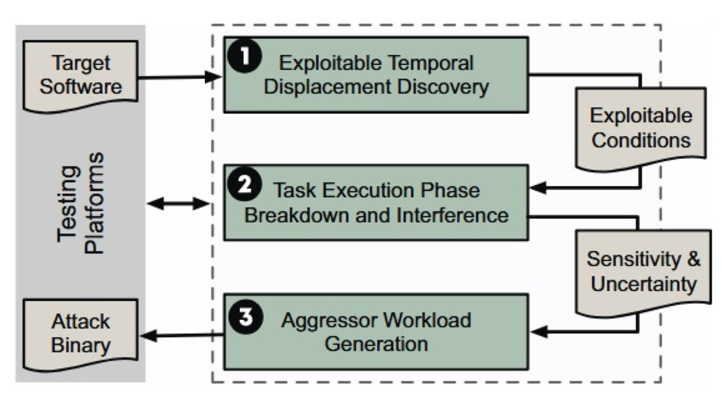
\includegraphics[width=0.80\columnwidth]
        {figures/timetrap.pdf}
    \caption{The workflow of TimeTrap. Reproduced from~\cite{li2024timetrap}.}
    \label{fig:timetrap}
\end{figure}
From a Mixed-Criticality Systems perspective, TimeTrap exposes a limitation of priority-based scheduling:
\begin{itemize}[nosep]
    \item Instead of directly competing for CPU time, the TimeTrap aggressor contends for shared architectural resources, such as caches and the memory bus;
    \item The resulting contention can stall safety-critical tasks, because priority assignment alone does not regulate interference on resources shared across cores;
    \item The attack demonstrates that software-level scheduling alone is insufficient to guarantee temporal isolation. Stronger isolation may be provided through \textit{Time and Space Partitioning (TSP)}, in which a partitioning hypervisor assigns separate execution windows and address spaces to different partitions, complemented by \textit{hardware-enforced partitioning} or regulation of shared resources such as caches and memory bandwidth.
\end{itemize}
Ultimately, this exposes a limitation of integrated multicore platforms: timing predictability cannot rely solely on priority-based CPU scheduling, but also requires explicit control of interference on shared hardware resources.
\\
\textbf{Claims and results} 
\\
The authors evaluated TimeTrap on eight real-world CPS applications using \textit{Hardware-in-The-Loop (HiTL)} simulations and physical tests on the OpenManipulator robotic arm and the Turtlebot3 robot. This allowed for a comprehensive analysis of several stages of the CPS pipeline, such as the perception, localization, planning, and control modules.
\\
The experiments confirmed that direct Denial-of-Service (DoS) attacks generally fail to cause critical physical damage. Both high-bandwidth and low-bandwidth DoS attempts triggered the systems' built-in fail-safe mechanisms or resulted in graceful degradation, such as safely halting the Turtlebot3 or causing only minimal deviations in the robotic arm.
\\
In contrast, TimeTrap successfully bypassed these safety checks by injecting targeted, fine-grained delays. This stealthy temporal displacement induced severe physical consequences: an attack on the robotic arm can cause deviations up to 30.1 cm and a collision; the Turtlebot3 computed incorrect paths based on stale costmaps; an Ardupilot drone showed severe velocity oscillations, leading to a crash.
\\
TimeTrap proved robust across ten different mission tasks, consistently achieving a success rate exceeding 60\% in both static and dynamic scenarios. Its effectiveness was even more pronounced in dynamic environments (reaching an 86\% success rate on the robotic arm), since these scenarios impose stricter timeliness requirements.
\\
Finally, the authors demonstrated that the impact of the attack heavily depends on the targeted shared resource, CPU budget, and task priority. Contention on cache and disk I/O proved significantly more effective than on network I/O, as the former are tightly coupled with the victim's computational phases. Consequently, the resulting temporal displacement scales proportionally with the CPU bandwidth and priority level assigned to the aggressor task.
\\
\textbf{Limitations}\\
The authors also noted several important limitations. First, the success of the attack strongly depends on the physical environment and the current state of the system. Since CPS outcomes are tied to real-world dynamics, the same interference pattern may have different effects depending on if the system is stationary, moving, or operating under changing conditions. In some cases, even a carefully modelled attack may take several seconds to destabilize the system.
\\
The second limitation is mainly constrained to local environments. TimeTrap relies on running the aggressor task on the same computing platform as the victim. This limits the TimeTrap extent compared with a remote attack. However, the authors note that in some systems there might be remotely exposed API that can trigger the interference workload indirectly. In that case, the aggressor would not need direct local code execution because the remote request could invoke a high-priority or resource-intensive path that creates the same kind of timing disruption.

\subsection{Purpose of the assignment}
The purpose of this assignment is not to reproduce the complete TimeTrap framework, but to investigate, on a smaller experimental scale, some of the timing-violation mechanisms and qualitative effects presented in the original paper. A complete reproduction would require automatic injection-point discovery, resource-oriented profiling, sensitivity analysis, and automatic aggressor-workload generation.
\\
Our work instead uses manually selected configurations and controlled perturbations to examine how a timing fault produces an internal temporal anomaly and if this anomaly propagates to control or mission-level behaviour.
The assignment includes two case studies. The \textbf{ArduPilot case study} primarily investigates the effects of different interference mechanisms, including indiscriminate resource saturation, explicit software delay injection, and a low-priority cache-contention workload.
The \textbf{TurtleBot3 case study} introduces explicit delays at different stages of the ROS Navigation pipeline, including localization, TF transmission, local-costmap production, and local-control execution. 
The two case studies do not provide a complete validation of TimeTrap or a general safety assessment. Their objective is to determine if some of the relations between timing perturbation, temporal displacement, data aging, control degradation, and mission-level effects can also be observed in reduced and controlled virtualized environments.
\\
\textbf{Learning objectives}\\ % POI DA DISCUTERNE NELLA PAGINA SELF-ASSESMENT
Through this assignment, we define the following shared learning objectives:
\begin{itemize}[nosep]
    \item \textbf{L0}: Understand the relation between performance interference, timing violations, temporal displacement, data freshness, and control degradation in Cyber-Physical Systems;
    \item \textbf{L1}: Design controlled, repeatable, and measurable real-time experiments using defined configurations, execution procedures, logging mechanisms, and quantitative metrics;
    \item \textbf{L2}: Compare how different perturbation mechanisms and different injection locations affect the timing and control behaviour of a Cyber-Physical System;
    \item \textbf{L3}: Analyze when an internal timing violation remains confined to the targeted software stage and when it propagates to control outputs, physical behaviour, or mission completion;
    \item \textbf{L4}: Critically evaluate if a reduced experimental reproduction supports some of the qualitative claims of the original work, while identifying the limitations introduced by simulation, virtualization, manual injection-point selection, and limited experimental coverage.
\end{itemize}

\subsection{Perimeter of investigation in the assignment}
\\
As introduced before, the complete TimeTrap workflow is beyond the perimeter of this project. The assignment is divided into two experimental case studies. For both case studies, the injection locations, delay values, and aggressor configuration are selected manually to reproduce the small-scale experiment.
\\
\textbf{ArduPilot case study} \\
The ArduPilot experiment is based on the Copter-4.0 version of the ArduPilot codebase. All tests are conducted using its Software-In-The-Loop (SITL) environment. Therefore, the experiment does not involve a physical drone or a flight-control hardware. A predefined mission is used in all configurations to make the different executions comparable and to observe the effects of interference under similar operating conditions.
\\
The ArduPilot case study is guided by the following research questions, which will be addressed in the results and discussion section:
\begin{itemize}[nosep]
    \item \textbf{A-Q0}: Does separating sensor emulation from the control thread change the normal timing and control behaviour of the system compared with the original baseline?     
    \item \textbf{A-Q1}: Does an indiscriminate Denial-of-Service workload mainly increase the wall-clock mission completion time, or does it also cause significant velocity-tracking deviations?
    \item \textbf{A-Q2}: Does targeted delay injection into the control path produce larger control-loop delays, greater navigation-state age, and higher velocity-tracking error than the baseline configurations?
    \item \textbf{A-Q3}: Can a low-priority cache-contention aggressor reproduce, at least qualitatively, the timing and control effects observed with explicit software delay injection?
\end{itemize}
\\ %qui ho dichiarato i 5 esperimenti fatti, segnando per ogni esperimento le research question in cui andrò ad utilizzare i risultati per comparare$
To answer these questions, the study considers both the original SITL architecture and a modified architecture in which sensor emulation is executed in a separate thread. Starting from these configurations, we evaluate the following experimental conditions:
\begin{itemize}[nosep]
    \item \textbf{A-E0}: An execution of the original SITL with logging instrumentation but without interference, which represents the main baseline [A-Q0][A-Q1];
    \item \textbf{A-E1}: An execution of the original SITL under a Denial-of-Service workload [A-Q1];
    \item \textbf{A-E2}: An execution of the modified SITL, with the sensor emulation separated from the control thread but without interference [A-Q0][A-Q2][A-Q3];
    \item \textbf{A-E3}: Two configurations of the modified SITL, with software delays of 30 ms and 50 ms injected into the AUTO waypoint-control path [A-Q2][A-Q3];
    \item \textbf{A-E4}: An execution of the modified SITL under interference generated by a low-priority cache-contention aggressor [A-Q3].
\end{itemize}
\\
The analysis focuses on observable timing and control indicators, including temporal displacement, velocity tracking error, and mission duration. These measurements are used to compare the different configurations and not to provide a complete safety assessment of ArduPilot.
\\
Furthermore, no direct equivalence is claimed between our SITL environment and the hardware-in-the-loop platforms used in the original study, or between the simulation results and the behaviour of the physical drone. The objective is limited to observing if some of the qualitative timing and control effects discussed in the paper can also appear in a smaller and controlled environment.
\\
\textbf{TurtleBot3 case study}\\
The TurtleBot3 case study is based on the ROS Noetic Navigation Stack and uses Gazebo 11 to simulate a TurtleBot3 Burger operating in the \texttt{turtlebot3\_world} environment. The experiments do not involve a physical robot or dedicated embedded navigation hardware. A predefined navigation task is used across the configurations to make the executions comparable and to observe the effects of timing perturbations under similar conditions.
\\
The TurtleBot3 case study is led by the following research questions, which are addressed in the results and comparative-analysis sections:
\begin{itemize}[nosep]
    \item \textbf{T-Q0}: Do the instrumented zero-delay configurations preserve the externally observable command timing and navigation behaviour of the clean TurtleBot3 baseline?
    \item \textbf{T-Q1}: Do controlled software delays produce measurable and increasing temporal displacement or data-age effects at the targeted navigation stage?
    \item \textbf{T-Q2}: To what extent do internal timing violations propagate to the \texttt{/cmd\_vel} stream and mission-level behaviour?
    \item \textbf{T-Q3}: At comparable delay levels, how does the injection location affect timing propagation, navigation availability, and observed safety-related outcomes?
\end{itemize}
To answer these questions, we manually selected injection points at different stages of the ROS Navigation pipeline. Starting from a clean baseline, we evaluated the following experimental configurations:
\begin{itemize}[nosep]
    \item \textbf{T-E0}: An execution of the unmodified ROS Navigation Stack without source-level delay instrumentation, used as the clean navigation baseline [T-Q0];
    \item \textbf{T-E1}: A set of configurations in which a controlled software delay is introduced before the publication of the AMCL pose estimate [T-Q0][T-Q1][T-Q2][T-Q3];
    \item \textbf{T-E2}: A set of configurations in which the AMCL map-to-odometry transform is delayed immediately before its transmission through the TF tree [T-Q0][T-Q1][T-Q2];
    \item \textbf{T-E3}: A set of configurations in which the local-costmap producer task is delayed immediately before updating the map [T-Q0][T-Q1][T-Q2][T-Q3];
    \item \textbf{T-E4}: A set of configurations in which the invocation of the local planner is delayed inside the \texttt{move\_base} control cycle [T-Q0][T-Q1][T-Q2][T-Q3];
    \item \textbf{T-E5}: A set of configurations in which the suspension is introduced at the beginning of the DWA controller execution [T-Q0][T-Q1][T-Q2][T-Q3].
\end{itemize}
Each instrumented experiment includes a zero-delay condition that retains the corresponding source-level timing and logging code without applying an intentional suspension. These conditions are used as matched references for the delayed executions, while T-E0 is used to determine if the instrumentation substantially changes nominal navigation behaviour.
\\
The analysis combines stage-specific internal timing measurements with externally observable navigation indicators.
\\
These measurements are used to compare the timing and behavioural effects of the different injection locations and not to provide a complete safety assessment of TurtleBot3. Moreover, no direct equivalence is claimed between the adopted Gazebo and virtual environments and the physical TurtleBot3 platform evaluated in the original work. The experiments use explicit source-level suspensions rather than TimeTrap-generated resource contention and are conducted in a static simulated environment.
\\
The objective is limited to determining if some of the qualitative temporal displacement and propagation effects discussed in the original paper can also be observed in a smaller and more controlled navigation scenario.

\section{Work product}

\subsection{ArduPilot case study} 
\subsubsection{Technical choices made in the case study}
\leavevmode\par
\noindent \textbf{Experimental environment}

\noindent We ran all ArduPilot experiments in the same VMware virtual machine running Ubuntu 22.04 LTS. We assigned four virtual CPUs, 8~GB of RAM, and a 50~GB virtual disk to the virtual machine.

\noindent We used the Copter-4.0 version of ArduPilot ~\cite{ardupilot_copter4.0} and executed it in its Software-In-The-Loop (SITL) environment. SITL allowed us to test the flight-control software without using a physical drone or dedicated flight-control hardware.

\noindent We used the same virtual machine configuration for all experimental conditions. This choice gave us a consistent software environment and reduced variations caused by different operating-system or tool configurations. It also allowed us to restore a known environment during development.

\noindent Virtualization, however, introduces an additional scheduling layer between the guest threads, the virtual CPUs, and the physical processor. Host activity and hypervisor scheduling may affect wall-clock measurements. For this reason, our results describe the behaviour observed in the adopted virtualized environment and cannot be directly generalized to dedicated flight-control hardware.

\noindent Table~\ref{tab:ardupilot-env} summarizes the main characteristics of the experimental platform.

\begin{table}[t]
    \centering
    \caption{ArduPilot experimental environment.}
    \label{tab:ardupilot-env}
    \small
    \begin{tabular}{ll}
        \toprule
        Component & Configuration \\
        \midrule
        Virtualization platform & VMware  \\
        Guest operating system & Ubuntu 22.04 LTS \\
        Guest Linux kernel & 6.8.0-124-generic \\
        Host processor &
            AMD Ryzen 5 3500U \\
        Host cores / logical CPUs & 4 / 8 \\
        Guest-visible CPUs & 4 \\
        Guest-visible L3 cache & 4 MiB \\
        Guest memory & 8 GB \\
        Target software & ArduPilot Copter-4.0 \\
        Simulation environment & SITL \\
        GCC version & 11.4.0 \\
        Python version & 3.10.12 \\
        stress-ng version & 0.13.12 \\
        \bottomrule
    \end{tabular}
\end{table}

\noindent \textbf{Common mission and controlled conditions} \\
\noindent We used the same predefined mission for all experimental configurations. We kept the same initial position, waypoint sequence, simulated vehicle model, ArduPilot parameter set, and AUTO flight mode. We also used the same procedure to load, arm, start, and terminate the mission. Each experiment was run three times.

\noindent These choices allowed us to compare the configurations over the same simulated flight and reduced the influence of variables unrelated to the investigated timing perturbations.

\noindent We selected the transition from navigation index 2 to navigation index 3 as the critical mission phase. As shown in Figure~\ref{fig:ardupilot-mission}, this transition requires a
relatively sharp change in direction. We therefore considered it a suitable phase in which delayed control computations could produce a visible velocity or trajectory deviation. We used this transition as the activation point for the explicit software delay in A-E3 and for the cache-contention aggressor in A-E4. This choice follows the general sharp-turn scenario discussed in the original work, but we do not claim that our waypoint geometry or activation instant exactly reproduces the authors' mission.

\begin{figure}[t]
    \centering
    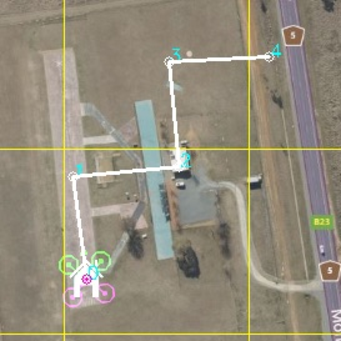
\includegraphics[width=0.50\columnwidth]
        {figures/ardupilot-mission.pdf}
    \caption{Predefined ArduPilot mission: the transition from navigation index 2 to 3 shows the critical phase used in A-E3 and A-E4.}
    \label{fig:ardupilot-mission}
\end{figure}

\noindent More detailed instructions for reproducing each experiment are available in our repository. Each experiment is provided in a dedicated branch containing a customized \texttt{README.md} file ~\cite{repo-github}.

\noindent \textbf{Logging and recorded measurements} \\
\noindent We implemented a common custom logger in \texttt{Copter.cpp} and used it in every experimental configuration. The logger creates the file \texttt{exp\_log.csv} during \texttt{Copter::setup()} and records data only while the motors are armed, resulting in a CSV that covers the active flight phase.

\noindent We collected one sample during each invocation of 

\noindent \texttt{Copter::fast\_loop()}, whose nominal execution frequency is 400~Hz. We recorded both simulation time and wall-clock time:
\begin{itemize}[nosep]
    \item \emph{Simulation time}: It represents the progression of the simulated physical system and advances when SITL completes new flight-dynamics steps;
    \item \emph{Wall-clock time}: It represents the actual time elapsed inside the virtual machine, including time spent sleeping, waiting for CPU execution, or being delayed by other workloads.
\end{itemize}

\noindent We kept the two time domains separate because the simulated system does not necessarily advance at the same rate as wall-clock time. This difference becomes particularly relevant when we inject a sleep or execute an external stress workload.

\noindent Table~\ref{tab:ardupilot-measurements} groups the recorded CSV fields and their purpose.

\begin{table*}[t]
    \centering
    \caption{Measurements recorded by the custom ArduPilot logger.}
    \label{tab:ardupilot-measurements}
    \footnotesize
    \begin{tabular}{
        p{0.18\textwidth}
        p{0.32\textwidth}
        p{0.44\textwidth}}
        \toprule
        Measurement group &
        CSV fields &
        Information provided \\
        \midrule

        Control-loop timing &
        \texttt{SIM\_TIME\_US},
        \texttt{WALL\_TIME\_US},
        \texttt{CONTROL\_DT\_SIM\_US},
        \texttt{CONTROL\_DT\_WALL\_US} &
        We recorded when each control iteration started and the
        interval since the previous iteration. These fields show
        if the control thread started later than in the nominal
        execution. \\

        Nominal-period excess &
        \texttt{CONTROL\_OVERRUN\_SIM\_US},
        \texttt{CONTROL\_OVERRUN\_WALL\_US} &
        We recorded the positive difference between the measured
        control-loop interval and the nominal 2500-$\mu$s period.
        We used these values only as diagnostic indicators, not as
        evidence of formally defined deadline misses. \\

        INS update timing &
        \texttt{INS\_UPDATE\_US},
        \texttt{INS\_DT\_US} &
        We recorded the timestamp of the latest processed inertial
        sensor update and the interval between consecutive updates.
        These values indicate how regularly the control thread
        refreshed its inertial state. \\

        Sensor-producer timing &
        \texttt{PRODUCER\_SIM\_US},
        \texttt{PRODUCER\_WALL\_US},
        \texttt{AGE\_SIM\_US},
        \texttt{AGE\_WALL\_US} &
        We recorded when the separated sensor thread completed its
        latest update and how old that update was when the control
        iteration started. These fields apply only to A-E2, A-E3,
        and A-E4. \\

        Navigation-state freshness &
        \texttt{INS\_BEFORE\_WPNAV\_US},
        \texttt{INS\_AFTER\_WPNAV\_US},
        \texttt{INS\_UPDATED\_DURING\_WPNAV},
        \texttt{STATE\_AGE\_AT\_WPNAV\_US} &
        We recorded if the processed INS state changed during
        the flight-mode update and how old that state was when the
        update completed. These fields allow us to distinguish recent
        sensor production from the use of an older processed control
        state. \\

        Flight-mode elapsed time &
        \texttt{WPNAV\_ELAPSED\_WALL\_US} &
        We measured the wall-clock duration of the flight-mode update
        containing \texttt{wp\_nav->update\_wpnav()}. In A-E3, this
        interval also contains the injected software sleep. \\

        Mission progress &
        \texttt{NAV\_INDEX},
        \texttt{WP\_DISTANCE\_CM} &
        We recorded the active navigation index and the remaining
        distance from the current waypoint. We used these fields to
        identify and align the critical mission phase. \\

        Horizontal velocity &
        \texttt{REF\_VEL\_N},
        \texttt{SIM\_VEL\_N},
        \texttt{REF\_VEL\_E},
        \texttt{SIM\_VEL\_E} &
        We recorded the North and East components of the target and
        estimated vehicle velocities, in centimetres per second.
        These fields support the evaluation of velocity-tracking
        performance. \\
        \bottomrule
    \end{tabular}
\end{table*}

\noindent In addition to the custom CSV, we collected the native ArduPilot BIN log for each final execution. We used the BIN log to inspect the vehicle's trajectory and altitude.

\noindent The logger periodically flushes its buffered output to reduce the amount of data lost if SITL terminates unexpectedly. Since the instrumentation performs timestamp acquisition, value extraction, and formatted file output inside the control thread, it introduces some execution overhead. However, we applied the same common logger to all configurations, including the two baseline configurations, so that this overhead is part of every comparison.

\noindent \textbf{Evaluation metrics} \\
\noindent We calculated every metric separately for each run. We analyze every run by taking in consideration two navigation windows:
\begin{itemize}[nosep]
    \item \textit{Complete navigation window}: From the beginning of \texttt{NAV\_INDEX = 1} to \texttt{NAV\_INDEX = 4};
    \item \textit{Critical navigation window}: Starts when \texttt{NAV\_INDEX} changes from 2 to 3.
\end{itemize}

\noindent We measured the navigation duration using both wall-clock and simulation time:
\begin{align}
D_{\mathrm{wall}} &=
\frac{
\texttt{WALL\_TIME\_US}_{\mathrm{end}}-
\texttt{WALL\_TIME\_US}_{\mathrm{start}}
}{10^6}, \\
D_{\mathrm{sim}} &=
\frac{
\texttt{SIM\_TIME\_US}_{\mathrm{end}}-
\texttt{SIM\_TIME\_US}_{\mathrm{start}}
}{10^6}.
\end{align}

\noindent For each sample \(k\), we calculated the horizontal velocity error as:
\begin{align}
e_N(k) &=
\texttt{REF\_VEL\_N}(k)-\texttt{SIM\_VEL\_N}(k), \\
e_E(k) &=
\texttt{REF\_VEL\_E}(k)-\texttt{SIM\_VEL\_E}(k), \\
e_v(k) &= \sqrt{e_N(k)^2+e_E(k)^2}.
\end{align}

\noindent We summarized the velocity error using its root mean square error and maximum value:
\begin{align}
\mathrm{RMSE}_v &=
\sqrt{\frac{1}{N}\sum_{k=1}^{N}e_v(k)^2}, \\
e_{v,\max} &= \max_{1\leq k\leq N}e_v(k).
\end{align}

\noindent We measured the wall-clock control interval and the elapsed time of the control section containing the waypoint update as:
\begin{align}
T_{\mathrm{control}}(k) &=
\frac{\texttt{CONTROL\_DT\_WALL\_US}(k)}{1000}, \\
T_{\mathrm{wp}}(k) &=
\frac{\texttt{WPNAV\_ELAPSED\_WALL\_US}(k)}{1000}.
\end{align}

\noindent Both values are expressed in milliseconds.

\noindent We used the age of the processed navigation state at the point of use as the temporal displacement metric:
\begin{equation}
TD_{\mathrm{state}}(k)=
\frac{\texttt{STATE\_AGE\_AT\_WPNAV\_US}(k)}{1000}.
\end{equation}

\noindent For configurations with a separate sensor thread, we also measured the age of its latest update:
\begin{equation}
A_{\mathrm{producer}}(k)=
\frac{\texttt{AGE\_SIM\_US}(k)}{1000}.
\end{equation}

\noindent A low producer age together with a high state temporal displacement means that the sensor thread produced recent updates while the controller used an older processed state.

\noindent For timing and age measurements, we reported the mean and maximum values inside each analysis window. We first calculated every metric for each individual run and then reported the mean and sample standard deviation across the three runs as \(\overline{M}\pm s_M\).

\subsubsection{Design and results of the (small-scale) case study}
\leavevmode\par
\noindent \textbf{Experimental configurations overview} \\
\noindent We organized the ArduPilot case study into five experimental configurations: Table~\ref{tab:ardupilot-experiments} summarizes the configurations. 

\begin{table*}[t]
    \centering
    \caption{ArduPilot experimental configurations.}
    \label{tab:ardupilot-experiments}
    \small
    \begin{tabular}{lllll}
        \toprule
        ID &
        SITL architecture &
        Scheduling configuration &
        Perturbation &
        Experimental role \\
        \midrule

        A-E0 &
        Original &
        - &
        None &
        Instrumented original baseline \\

        A-E1 &
        Original &
        - &
        CPU, cache, and memory saturation &
        Indiscriminate-interference case \\

        A-E2 &
        Modified architecture &
        FIFO 80/60 &
        None &
        Modified-architecture baseline \\

        A-E3-30 &
        Modified architecture &
        FIFO 80/60 &
        30-ms control-thread delay &
        Moderate explicit delay \\

        A-E3-50 &
        Modified architecture &
        FIFO 80/60 &
        50-ms control-thread delay &
        Stronger explicit delay \\

        A-E4 &
        Modified architecture &
        FIFO 80/60/20 &
        Cache-contention aggressor &
        Resource-interference case \\

        \bottomrule
    \end{tabular}
\end{table*}

\noindent \textbf{A-E0: Instrumented original baseline} \\
\noindent In A-E0, we preserved the original Copter-4.0 SITL execution architecture and ran the predefined mission without an external perturbation. In the original architecture, the main SITL execution flow advances both the simulated physical system and the flight-control software. When the main thread waits for the simulation clock,
\texttt{SITL\_State::wait\_clock()} invokes \texttt{\_fdm\_input\_step()}. This function advances the flight-dynamics model, updates the simulated vehicle and sensor interfaces, executes the associated timer events, and advances the synthetic simulation clock. Sensor production and control execution are coupled in the same overall execution flow. If this flow is delayed, the simulated physical system and the flight-control computation are delayed together.

\noindent We only added the common logging instrumentation described in the previous section. 

\noindent We used A-E0 as the reference for evaluating A-E1 and for determining if the architectural changes introduced in A-E2 altered the nominal behaviour of SITL.

\begin{table*}[t]
    \centering
    \caption{ArduPilot results. Values report the mean and sample
    standard deviation across three runs. Velocity values are in
    cm/s; timing and age values are in ms.}
    \label{tab:ardupilot-results}
    \scriptsize
    \setlength{\tabcolsep}{3.5pt}

    \begin{tabular}{@{}lrrrrrr@{}}
        \toprule
        \multicolumn{7}{l}{
        \textbf{Complete navigation window}
        }\\
        \midrule
        Experiment &
        Success &
        \(D_{\mathrm{wall}}\) &
        \(D_{\mathrm{sim}}\) &
        \(\mathrm{RMSE}_{v,\mathrm{nav}}\) &
        \(\mathrm{RMSE}_{\mathrm{NAV3}}\) &
        \(e_{\max,\mathrm{NAV3}}\) \\
        \midrule

        A-E0 &
        3/3 &
        \(57.28 \pm 0.42\) &
        \(57.01 \pm 0.02\) &
        \(46.29 \pm 0.03\) &
        \(48.99 \pm 0.08\) &
        \(104.78 \pm 0.09\) \\

        A-E1 &
        3/3 &
        \(57.55 \pm 0.51\) &
        \(57.02 \pm 0.04\) &
        \(46.29 \pm 0.04\) &
        \(49.02 \pm 0.10\) &
        \(105.15 \pm 0.31\) \\

        A-E2 &
        3/3 &
        \(104.22 \pm 2.04\) &
        \(57.77 \pm 0.05\) &
        \(45.96 \pm 0.06\) &
        \(48.57 \pm 0.14\) &
        \(104.80 \pm 0.81\) \\

        A-E3-30 &
        3/3 &
        \(108.65 \pm 2.59\) &
        \(60.94 \pm 0.32\) &
        \(49.90 \pm 0.27\) &
        \(63.10 \pm 0.89\) &
        \(232.86 \pm 19.24\) \\

        A-E3-50 &
        3/3 &
        \(133.85 \pm 2.38\) &
        \(74.78 \pm 1.46\) &
        \(122.94 \pm 25.08\) &
        \(193.03 \pm 40.49\) &
        \(810.42 \pm 138.30\) \\

        A-E4 &
        3/3 &
        \(99.74 \pm 2.21\) &
        \(57.67 \pm 0.08\) &
        \(46.02 \pm 0.05\) &
        \(48.67 \pm 0.08\) &
        \(104.76 \pm 0.38\) \\

        \bottomrule
    \end{tabular}

    \vspace{1.2ex}

    \begin{tabular}{@{}lrrrrrr@{}}
        \toprule
        \multicolumn{7}{l}{
        \textbf{Critical navigation window}
        }\\
        \midrule
        Experiment, window &
        \(\mathrm{RMSE}_{v}\) &
        \(e_{v,\max}\) &
        \(\overline{T}_{\mathrm{control}}\) &
        \(\overline{T}_{\mathrm{wp}}\) &
        \(\overline{TD}_{\mathrm{state}}\) &
        \(\overline{A}_{\mathrm{producer}}\) \\
        \midrule

        A-E2, 200 cycles &
        \(24.58 \pm 0.23\) &
        \(38.67 \pm 0.05\) &
        \(4.545 \pm 0.062\) &
        \(0.015 \pm 0.001\) &
        \(0.171 \pm 0.011\) &
        \(0.046 \pm 0.007\) \\

        A-E3-30, 200 cycles &
        \(113.14 \pm 9.63\) &
        \(210.09 \pm 13.14\) &
        \(32.214 \pm 0.088\) &
        \(30.395 \pm 0.051\) &
        \(17.254 \pm 0.295\) &
        \(0.057 \pm 0.005\) \\

        A-E3-50, 200 cycles &
        \(115.50 \pm 8.34\) &
        \(216.56 \pm 24.97\) &
        \(52.154 \pm 0.108\) &
        \(50.388 \pm 0.029\) &
        \(28.175 \pm 0.389\) &
        \(0.040 \pm 0.015\) \\

        A-E2, 6 s &
        \(76.72 \pm 0.10\) &
        \(104.80 \pm 0.81\) &
        \(4.547 \pm 0.070\) &
        \(0.014 \pm 0.002\) &
        \(0.202 \pm 0.017\) &
        \(0.055 \pm 0.010\) \\

        A-E4, 6 s &
        \(76.74 \pm 0.40\) &
        \(104.76 \pm 0.38\) &
        \(4.506 \pm 0.093\) &
        \(0.015 \pm 0.001\) &
        \(0.152 \pm 0.018\) &
        \(0.023 \pm 0.002\) \\

        \bottomrule
    \end{tabular}
\end{table*}

\noindent Table~\ref{tab:ardupilot-results} shows that all three A-E0 runs completed the mission with a low variation between runs. Wall-clock duration and simulation duration were almost equal
(\(57.28\) and \(57.01\)~s, respectively). The original coupled SITL architecture progressed approximately in real time. The velocity RMSE was \(46.29\)~cm/s over the complete navigation and \(48.99\)~cm/s during \texttt{NAV\_INDEX = 3}. The maximum error in this phase was around \(104.78\)~cm/s. These values define the repeatable baseline level observed for the selected mission. Temporal displacement and producer-age measurements are not applicable to this configuration.

\noindent \textbf{A-E1: Indiscriminate resource saturation} \\
\noindent In A-E1, we used the same original SITL architecture and logging instrumentation used in A-E0. We just introduced an external \texttt{stress-ng} workload to generate broad CPU, cache, and memory pressure inside the virtual machine.

\noindent We started the workload with:
\begin{verbatim}
stress-ng --cpu 4 --cache 4 --vm 2 --vm-bytes 1G
\end{verbatim}

\noindent The command creates four CPU stressors, four cache stressors, and two virtual-memory stressors.

\noindent We started the workload at the beginning of the run and kept it alive until the end. A-E1 does not target a specific ArduPilot execution phase or control function. Instead, it generates indiscriminate resource saturation across the virtual machine.

\noindent We designed this configuration to evaluate if broad resource saturation mainly increases the time required to execute the mission or also produces relevant velocity and trajectory deviations.

\noindent As reported in Table~\ref{tab:ardupilot-results}, all three A-E1 runs
completed the mission while the CPU, cache, and memory workload was
active. Wall-clock duration remained close to simulation duration
(\(57.55\) and \(57.02\)~s). This indicates that the simulated
physical system and the control software continued to progress
together under the external load.
The complete-navigation velocity RMSE was \(46.29\)~cm/s. During
\texttt{NAV\_INDEX = 3}, the RMSE was \(49.02\)~cm/s and the maximum
instantaneous error was approximately \(105.15\)~cm/s. The small
standard deviations show that the three executions produced a
consistent response.
The workload produced no mission failure or unstable vehicle response in
the recorded runs.

\noindent \textbf{A-E2: Modified SITL baseline with separated sensor emulation} \\
\noindent In A-E2, we modified the original SITL architecture. As identified by the authors, to emulate the function of ArduPilot's normal flight mode, it is necessary to modify the SITL simulation environment by separating the advancement of the simulated physical system and sensor interfaces from the main control thread.

\noindent First, we removed the original call to \texttt{\_fdm\_input\_step()} from the control-side implementation of \texttt{SITL\_State::wait\_clock()}. The control thread continues to wait for the synthetic simulation clock, but it no longer advances the flight-dynamics model itself.

\noindent Second, we created a separate thread during SITL initialization. This thread executes \texttt{SITL\_State::\_sensor\_thread()}, whose main loop is:
\begin{verbatim}
while (!Scheduler::_should_exit) {
    // advances the flight-dynamics model
    // updates the simulated vehicle
    // executes the related timer events
    // advances the synthetic simulation clock
    _fdm_input_step();
    // prevents the high-priority thread from 
    // continuously executing without voluntarily blocking
    usleep(1000);
}
\end{verbatim}
\noindent The one-millisecond sleep was used only as a pacing mechanism. It does not define an exact one-kilohertz sensor period, because the actual wake-up time depends on guest and hypervisor scheduling.

\noindent We configured the sensor-emulation thread with the Linux \texttt{SCHED\_FIFO} policy and priority 80, and the main control thread with the same policy and priority 60. We verified these settings at runtime.  

\noindent We applied the scheduling configuration directly in the modified \texttt{SITL\_State.cpp}. We defined a helper function that initialized a POSIX \texttt{sched\_param} structure with the requested priority and called \texttt{pthread\_setschedparam(pthread\_self(), SCHED\_FIFO, \&param)}. The call to \texttt{pthread\_setschedparam()} affects only the thread that invokes it. So, we called the helper separately from the sensor thread and from the control thread, assigning priorities 80 and 60, respectively. Other ArduPilot threads were not modified by these calls. In particular, the sensor thread invoked this helper with priority 80 when entering \texttt{\_sensor\_thread()}. This ordering follows the priority relation described in the original ArduPilot case study, where sensor and I/O activities have a higher priority than the control computation.

\noindent Under \texttt{SCHED\_FIFO}, when runnable threads compete for the same CPU, the scheduler selects the thread with the highest real-time priority. A running FIFO thread continues until it blocks, yields, or is preempted by a higher-priority thread. Therefore, a ready sensor thread can preempt the control thread when they compete for the same virtual CPU. The sensor thread voluntarily blocks through \texttt{usleep(1000)}, preventing it from continuously occupying a processor and allowing the lower-priority control thread to execute.
We selected \texttt{SCHED\_FIFO} instead of \texttt{SCHED\_RR} because the relevant threads have different priorities. The round-robin time quantum only adds time sharing between runnable threads at the same priority, which our configuration does not require.

\noindent We did not introduce any delay or external aggressor in A-E2. We used this configuration to determine if the modified architecture preserved the nominal mission behaviour and we used it as the direct baseline for A-E3 and A-E4.

\noindent Table~\ref{tab:ardupilot-results} shows that all three A-E2 runs completed the mission and produced consistent measurements. The simulated navigation lasted \(57.77\)~s, but its execution required \(104.22\)~s of wall-clock time. The modified two-thread SITL operated below real time in the virtual machine. This slowdown did not produce a relevant control degradation. The complete-navigation velocity RMSE was \(45.96\)~cm/s, while the RMSE during \texttt{NAV\_INDEX = 3} was \(48.57\)~cm/s. The maximum error during this phase remained close to \(104.80\)~cm/s.
The critical windows in Table~\ref{tab:ardupilot-results} also show
stable control timing. The mean control interval remained close to
\(4.55\)~ms, and the control section containing the waypoint update
required approximately \(0.015\)~ms. State temporal displacement and producer age remained below one millisecond.  These measurements show that the separated threads remained
temporally aligned during the baseline execution. The sensor thread
produced recent updates, and the controller used recently processed
state. A-E2 provides the baseline for the modified architecture.

\noindent \textbf{A-E3: Explicit software delay injection}

\noindent A-E3 uses the modified architecture and the scheduling configuration introduced in A-E2. In this experiment, we inserted a controlled software delay into the main control thread.

\noindent We placed the delay inside \texttt{ModeAuto::wp\_run()}, immediately before \texttt{wp\_nav->update\_wpnav()}. We selected this point because the control thread reaches it after processing the inertial and navigation state for the current fast-loop iteration, but before the AUTO waypoint controller uses that processed state.

\noindent  The execution order is:
\begin{verbatim}
ins.update()
read_AHRS()
read_inertia()
ModeAuto::wp_run()
    usleep(...)
    wp_nav->update_wpnav()
\end{verbatim}
\noindent The \texttt{usleep()} call suspends only the control thread. During this suspension, the independent sensor-emulation thread continues to advance the simulated physical system and update the simulated sensor interfaces.

\noindent When the control thread wakes up, it starts from the same program location and directly invokes \texttt{wp\_nav->update\_wpnav()}. It does not repeat \texttt{ins.update()}, \texttt{read\_AHRS()}, or \texttt{read\_inertia()} before doing so.

\noindent As a result, newer simulated sensor updates may exist when the control thread wakes up, while the waypoint controller still uses the processed INS/AHRS/navigation state computed before the delay. We designed A-E3 to create and measure this temporary mismatch between sensor progression and control-state freshness.

\noindent We activate the delay when the mission navigation index changes from 2 to 3. We then apply it during 200 consecutive invocations of \texttt{ModeAuto::wp\_run()}.

\noindent We evaluate two delay magnitudes:
\begin{itemize}[nosep]
    \item \textbf{A-E3-30}: We call \texttt{usleep(30000)}, requesting a 30-ms wall-clock suspension;
    \item \textbf{A-E3-50}: We call \texttt{usleep(50000)}, requesting a 50-ms wall-clock suspension.
\end{itemize}

\noindent All three A-E3-30 runs completed the mission, as shown in
Table~\ref{tab:ardupilot-results}. The complete-navigation velocity
RMSE increased to \(49.90\)~cm/s. During the complete
\texttt{NAV\_INDEX = 3} phase, it reached \(63.10\)~cm/s, with a
maximum error of \(232.86\)~cm/s. The effect was concentrated around the mission phase in which we activated the delay.
During the 200 delayed iterations, the mean control interval was
\(32.21\)~ms. The measured control section containing the waypoint
update required \(30.40\)~ms on average. These results confirm that the 30-ms delay was applied consistently.
The same window produced a velocity RMSE of \(113.14\)~cm/s and a
maximum error of \(210.09\)~cm/s. At the same time, mean state
temporal displacement increased to \(17.25\)~ms, while mean producer age remained only \(0.057\)~ms.
The low producer age shows that the sensor thread continued advancing and publishing recent updates. The higher state age shows that the waypoint controller still used navigation state processed before the control-thread suspension.

\noindent Table~\ref{tab:ardupilot-results} reports that all three A-E3-50 runs completed the mission, but the stronger delay produced a large change in the vehicle response. 
During the 200 delayed iterations, the mean control interval was
\(52.15\)~ms, and the control section containing the waypoint update required \(50.39\)~ms. These values closely match the requested 50-ms sleep and show that the timing injection remained repeatable across the three runs.
The mean state temporal displacement reached \(28.18\)~ms, while the mean producer age remained only \(0.040\)~ms. The sensor thread continued to provide recent updates, but the controller used older processed state.
The complete-navigation velocity RMSE reached \(122.94\)~cm/s. 
Within the 200 delayed cycles, the velocity RMSE was
\(115.50\)~cm/s and the maximum error was \(216.56\)~cm/s.
When we considered the complete \texttt{NAV\_INDEX = 3} phase,
the RMSE increased to \(193.03\)~cm/s and the maximum error reached
\(810.42\)~cm/s.
Since the complete \texttt{NAV\_INDEX = 3} phase includes also the initial 200 delayed cycles, these values show that the largest velocity deviations occurred after the delay-injection window. While the software sleep had already ended, the vehicle had reached a disturbed position and motion state and still had to recover towards the planned path. The later errors are consistent with the delay affecting not only the initial turn, but also the subsequent vehicle response and recovery.
The control timing was highly repeatable across the three runs, as
shown by the small standard deviations of the measured delay.
The larger variation in the velocity metrics indicates that the same timing disturbance produced less repeatable physical responses, depending on the vehicle state reached during the critical phase.

\noindent \textbf{A-E4: Low-priority cache-contention aggressor}

\noindent A-E4 uses the same modified SITL architecture and the same sensor and control scheduling configuration introduced in A-E2. In this experiment we use an external cache-oriented workload. When the mission navigation index changes from 2 to 3, the ArduPilot control path creates the trigger file:
\begin{verbatim}
/dev/shm/timetrap_e4.trigger
\end{verbatim}
\noindent Before starting the mission, we launch a shell script that waits for this file. When the script detects the trigger, it executes:
\begin{verbatim}
taskset -c 0 chrt -f 20 stress-ng \
    --cache 1 \
    --cache-level 3 \
    --timeout 6s \
    --metrics-brief
\end{verbatim}

\noindent The command configures the workload as follows:
\begin{itemize}[nosep]
    \item \texttt{taskset -c 0} restricts the aggressor to guest virtual CPU~0;
    \item \texttt{chrt -f 20} assigns \texttt{SCHED\_FIFO} policy and priority 20;
    \item \texttt{--cache 1} creates one cache stressor;
    \item \texttt{--cache-level 3} requests activity directed at the guest-visible level-3 cache;
    \item \texttt{--timeout 6s} limits the workload to six seconds;
    \item \texttt{--metrics-brief} prints a short execution summary.
\end{itemize}

\noindent The complete priority ordering in A-E4 is:
\begin{equation}
P_{\mathrm{sensor}}=80
>
P_{\mathrm{control}}=60
>
P_{\mathrm{aggressor}}=20.
\end{equation}

\noindent As done by the authors, we assigned the aggressor a lower priority than the sensor and control threads so that it could not directly dominate them through fixed-priority CPU scheduling. We instead wanted it to affect their execution through pressure on shared cache and memory-system resources.

\noindent This configuration approximates only the final resource-interference stage of TimeTrap. We manually selected the targeted resource, priority, processor affinity, activation phase, and duration. We did not reproduce TimeTrap's automatic profiling, sensitivity analysis, or aggressor synthesis.

\noindent Virtualization also limits the interpretation of this experiment. VMware controls the mapping between guest virtual CPUs and physical host cores. Therefore, restricting the aggressor to guest virtual CPU~0 does not guarantee a fixed mapping to a specific physical core or a particular physical last-level cache. For these reasons, we use A-E4 as a qualitative resource-contention experiment. 

\noindent All three A-E4 runs completed the mission and showed low
variation, as reported in Table~\ref{tab:ardupilot-results}. The
simulated navigation lasted \(57.67\)~s and required \(99.74\)~s of
wall-clock time. The modified SITL continued to execute
below real time.
The complete-navigation velocity RMSE was \(46.02\)~cm/s. During
\texttt{NAV\_INDEX = 3}, it was \(48.67\)~cm/s, and the maximum error was \(104.76\)~cm/s. No large or unstable vehicle response appeared in the three runs.
During the six-second aggressor window, the mean control interval was \(4.51\)~ms. The section containing the targeted waypoint update required only \(0.015\)~ms on average. Mean state temporal displacement remained
\(0.152\)~ms, while mean producer age was \(0.023\)~ms. Both the
produced sensor data and the processed navigation state remained recent.
The velocity RMSE in the same six-second window was \(76.74\)~cm/s, with a maximum error of \(104.76\)~cm/s. The timing and age measurements do not show a sustained delay in the control path.
Under the selected scheduling and virtualized hardware
configuration, the low-priority cache aggressor did not create a
clear temporal displacement effect.

\subsubsection{Comparative analysis and answers to the research questions}

\noindent Table~\ref{tab:ardupilot-results} reports the quantitative results, while Figures~\ref{fig:ardupilot-trajectories} and~\ref{fig:ardupilot-altitude} show the observed flight response in A-E2 and A-E3 configurations. All configurations completed three runs out of three. However, mission completion only indicates that the vehicle reached the final waypoint condition; it does not exclude unsafe intermediate deviations, such as those observed in A-E3-50.

\begin{figure}[t]
    \centering
    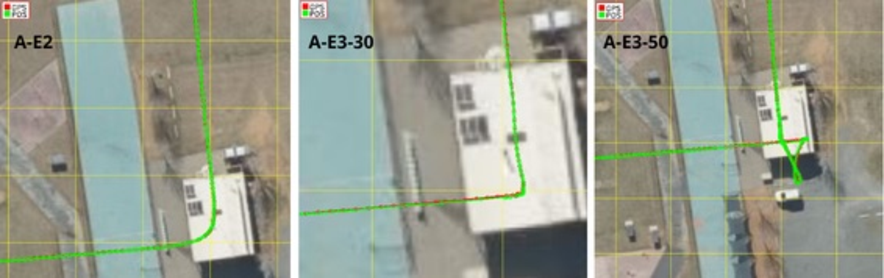
\includegraphics[width=1\columnwidth]
        {figures/A-E2-traiettoria.pdf}
    \caption{Horizontal trajectories around waypoint~3 for A-E2\_run1, A-E3-30\_run1, and A-E3-50\_run1.}
    \label{fig:ardupilot-trajectories}
\end{figure}

\begin{figure}[t]
    \centering
    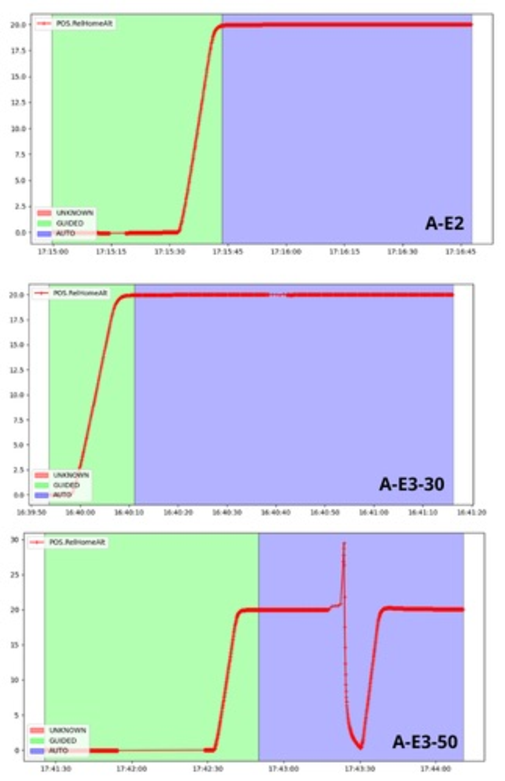
\includegraphics[width=0.50\columnwidth]
        {figures/A-E2.pdf}
    \caption{Altitude evolution for A-E2\_run1, A-E3-30\_run1, and A-E3-50\_run1.}
    \label{fig:ardupilot-altitude}
\end{figure}

\noindent \textbf{A-Q0. Partially.} \\
\noindent Separating sensor emulation from the control thread substantially changed wall-clock timing, but it did not produce a relevant degradation of nominal flight behaviour.

\noindent Compared with A-E0, A-E2 increased the wall-clock navigation duration from \(57.28 \pm 0.42\)~s to \(104.22 \pm 2.04\)~s. However, the simulation duration remained similar, changing from \(57.01 \pm 0.02\)~s to \(57.77 \pm 0.05\)~s. The modified configuration executed below real time in the virtual machine.

\noindent This wall-clock slowdown was not associated with worse nominal velocity tracking. The complete-navigation velocity RMSE changed only from \(46.29 \pm 0.03\)~cm/s in A-E0 to
\(45.96 \pm 0.06\)~cm/s in A-E2. In A-E2, producer age and state temporal displacement also remained below one millisecond, indicating that recent sensor updates and the recently processed navigation state were available during nominal execution.

\noindent A-E2 introduced thread separation, fixed-priority scheduling, and sensor-thread pacing at the same time. The comparison measures their combined effect. It does not determine which individual change caused the increase in wall-clock duration.

\noindent \textbf{A-Q1. No measurable effect was observed.} \\
\noindent Under the tested configuration, the indiscriminate resource-saturation
workload did not substantially increased mission duration or caused
a relevant velocity-tracking deviation.

\noindent A-E0 and A-E1 required \(57.28 \pm 0.42\)~s and
\(57.55 \pm 0.51\)~s of wall-clock time, respectively. Their
complete-navigation velocity RMSE was the same within the reported
precision, at approximately \(46.29\)~cm/s. During
\texttt{NAV\_INDEX = 3}, the RMSE changed only from
\(48.99 \pm 0.08\)~cm/s to \(49.02 \pm 0.10\)~cm/s, while the
maximum error remained close to \(105\)~cm/s.

\noindent The selected CPU, cache, and memory workload did not
produce a measurable change in the selected mission and control
metrics.

\noindent This result applies only to the selected \texttt{stress-ng} command,
virtual-machine configuration, and mission. It does not show that
indiscriminate resource saturation cannot affect ArduPilot under
different workloads or hardware conditions.

\noindent \textbf{A-Q2. Yes.} \\
\noindent Explicit delay injection into the control path produced a clear and
repeatable increase in control delay, navigation-state age, and
velocity-tracking error compared to A-E2.

\noindent During the matched 200-cycle window, the mean elapsed time of the
control section containing the targeted waypoint increased from
\(0.015 \pm 0.001\)~ms in A-E2 to
\(30.395 \pm 0.051\)~ms in A-E3-30 and
\(50.388 \pm 0.029\)~ms in A-E3-50. The corresponding mean control
intervals increased from \(4.545 \pm 0.062\)~ms to
\(32.214 \pm 0.088\)~ms and \(52.154 \pm 0.108\)~ms.

\noindent Mean state temporal displacement increased from
\(0.171 \pm 0.011\)~ms in A-E2 to
\(17.254 \pm 0.295\)~ms in A-E3-30 and
\(28.175 \pm 0.389\)~ms in A-E3-50. In contrast, mean producer age
remained close to zero in all three configurations. This means that recent updates from the sensor thread were available across the delayed iterations, while the waypoint controller used navigation state that was processed before the control-thread suspension.

\noindent The temporal effect was associated with a clear degradation in velocity tracking. During the complete
\texttt{NAV\_INDEX = 3} phase, velocity RMSE increased from
\(48.57 \pm 0.14\)~cm/s in A-E2 to
\(63.10 \pm 0.89\)~cm/s in A-E3-30 and
\(193.03 \pm 40.49\)~cm/s in A-E3-50. The maximum error increased
from approximately \(105\)~cm/s to \(233\)~cm/s and \(810\)~cm/s,
respectively.

\noindent Figure~\ref{fig:ardupilot-trajectories} shows the corresponding
physical behaviour. A-E2 followed the nominal turn, A-E3-30 followed a
wider path before recovering, and A-E3-50 produced a much larger
deviation. Figure~\ref{fig:ardupilot-altitude} shows that A-E2 and
A-E3-30 remained close to the nominal altitude, whereas A-E3-50
experienced a large altitude deviation, including a sharp drop
followed by recovery.

\noindent \textbf{A-Q3. No, under the tested configuration.} \\
\noindent The low-priority cache-contention aggressor did not reproduce the
timing and control effects observed with explicit software delay
injection.

\noindent During the matched six-second post-trigger window, the mean control
interval was \(4.547 \pm 0.070\)~ms in A-E2 and
\(4.506 \pm 0.093\)~ms in A-E4. The mean waypoint-control times were
also almost identical, at \(0.014 \pm 0.002\)~ms and
\(0.015 \pm 0.001\)~ms. State temporal displacement remained small,
with \(0.202 \pm 0.017\)~ms in A-E2 and
\(0.152 \pm 0.018\)~ms in A-E4.

\noindent The velocity RMSE values in the same window were also almost equal:
\(76.72 \pm 0.10\)~cm/s in A-E2 and
\(76.74 \pm 0.40\)~cm/s in A-E4. We did not observe a
sustained delay or a measurable temporal displacement effect on the
recorded control path.

\noindent The A-E4 aggressor ran at a lower fixed priority than both ArduPilot threads. It could affect them mainly through contention on shared cache or memory-system resources, rather than through direct fixed-priority preemption of the control thread. However, only the aggressor was pinned to a specific guest vCPU. The sensor and control threads were free to migrate across guest vCPUs, while VMware did not guarantee how guest vCPUs were mapped onto physical CPU cores.

\noindent This result does not show that cache-based or resource-based
interference is ineffective in general. It shows that the manually
configured A-E4 aggressor did not reproduce the A-E3
temporal displacement pattern under the tested virtualized setup.


\subsection{TurtleBot3 case study}
\subsubsection{Technical choices made in the case study} \\
\leavevmode\par
\noindent \textbf{Experimental environment} \\
We conducted the TurtleBot3 experiments in VMware and KVM virtual machines running Ubuntu 20.04.6 LTS. Both virtual machines used the same virtual-hardware allocation adopted for the ArduPilot experiments. The main difference between the two TurtleBot3 environments was the host processor: one was executed on an AMD Ryzen 5 9600X processor, while the other was executed on an Intel Core Ultra 7 155H processor.

\noindent Since some experiments were executed on different host processors, absolute
wall-clock measurements collected in one virtual machine are not assumed to
be directly interchangeable with those collected in the others. Differences in processors may affect callback execution and wake-up latency. Therefore, each delayed configuration is primarily evaluated against the corresponding zero-delay baseline collected in the same virtual machine.

\noindent The TurtleBot3 experiments used Gazebo Classic 11.15.1, the Gazebo 11 version integrated with ROS Noetic, to simulate the robot motion, its interaction with the environment, and the laser measurements. The TurtleBot3 Burger model and the \texttt{turtlebot3\_world} environment were provided by the official ROBOTIS TurtleBot3 simulation packages~\cite{turtle_simulation} for ROS Noetic, while the connection between Gazebo and ROS was provided by \texttt{gazebo\_ros\_pkgs}. The ROS Navigation Stack was obtained from the official \texttt{ros-planning/navigation} repository, using its \texttt{noetic-devel} branch, and was built from source in the catkin workspace~\cite{ros-planning}. This allowed us to instrument the selected AMCL, local-costmap, \texttt{move\_base}, and DWA controller operations.

\noindent The simulated environment allowed us to execute repeatable navigation tasks without using a physical robot and reduced the variability caused by mechanical conditions, physical sensor noise, and manual robot repositioning. However, Gazebo does not reproduce all hardware, communication, sensing, and actuation delays of a physical robot. Moreover, as already discussed for the ArduPilot case study, virtualization introduces an additional scheduling layer between the ROS processes, the guest virtual CPUs, and the physical processor. Therefore, our results describe the behaviour observed in the adopted virtualized environment and cannot be directly generalized to a physical TurtleBot3.

\noindent Table~\ref{tab:turtlebot-env} summarizes the main characteristics of the used platforms.

\begin{table}[t]
    \centering
    \caption{TurtleBot3 experimental environments.}
    \label{tab:turtlebot-env}
    \small
    \begin{tabular}{ll}
        \toprule
        Component & Configuration \\
        \midrule
        Virtualization platform
            & VMware / KVM \\

        Guest operating system
            & Ubuntu 20.04.6 LTS \\

        Guest Linux kernel
            & 5.15.0-139-generic \\

        Host processor
            & AMD Ryzen 5 9600X / Intel Core Ultra 7 155H \\

        Guest-visible CPUs
            & 4 \\

        Guest memory
            & 8 GB \\

        ROS distribution
            & ROS Noetic \\

        Simulation environment
            & Gazebo 11.15.1 \\

        Robot model
            & TurtleBot3 Burger \\

        Simulation world
            & turtlebot3\_world \\

        Navigation framework
            & ROS Navigation Stack \\
        \bottomrule
    \end{tabular}
\end{table}

\noindent \textbf{Common missions and controlled conditions} \label{sec:2.2.1} \\
We used the same predefined point-to-point navigation task for all TurtleBot3 experimental configurations. We kept the experimental procedure fixed within each experiment to reduce the influence of variables unrelated to the investigated timing perturbations. In particular, we used the same robot model, simulation world, map, initial pose, goal and run-termination criteria for all delay conditions executed.

\noindent The original study evaluated a physical TurtleBot3 in a physical environment. Moreover, the authors did not identify a specific mission phase in which the TurtleBot3 was particularly vulnerable to timing interference. For these reasons, we manually selected a navigation goal which forced the robot to move near obstacles and to perform relatively sharp turns along its path. Figure~\ref{fig:turtlebot-mission} shows the initial pose of the robot, the destination goal and the initial planned path. Moreover, the simulated environments remained static, and no dynamic obstacles were intentionally introduced. 

\begin{figure}[t]
    \centering
    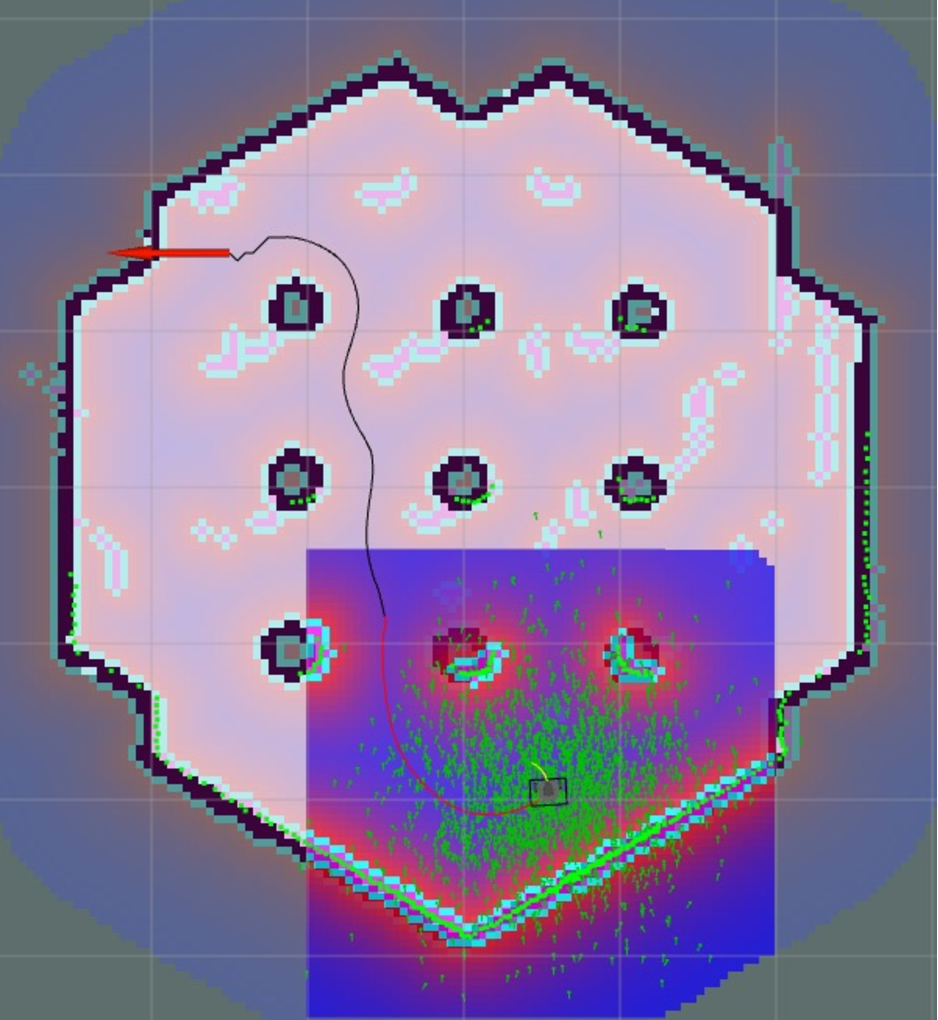
\includegraphics[width=0.5\columnwidth]
        {figures/turtlebot_mission.pdf}
    \caption{Predefined TurtleBot3 mission.}
    \label{fig:turtlebot-mission}
\end{figure}

\noindent For each run, we performed the following steps:
\begin{enumerate}[nosep]
    \item We launched Gazebo and the ROS Navigation Stack;
    \item We initialized the pose of the robot;
    \item We waited 3~ seconds for Gazebo and the navigation components to reach a stable operating state;
    \item We started recording the relevant system data and ROS messages;
    \item We published the navigation goal;
    \item We waited until the mission succeded, was aborted, or reached the predefined timeout;
    \item We stopped the data recording;
    \item We reset the simulation environment.
\end{enumerate}

\noindent More detailed instructions for reproducing each experiment are available in our repository. Each experiment is provided in a dedicated branch containing a customized \texttt{README.md} file ~\cite{repo-github}.

\noindent \textbf{Navigation pipeline and Delay Injection Points}\\
The TurtleBot3 navigation pipeline contains several \textit{producer-consumer} dependencies. It starts with the collection of the range measurements from the \textit{laser scanner} and the motion estimates from \textit{wheel odometry}. An Adaptive Monte Carlo Localization (AMCL) algorithm combines them with the static map, odometry information, and the TF transformation tree to estimate the robot pose. 

\noindent The localization and sensor information are then used by the local and global costmaps. The \textit{global costmap} represents the environment over the area used for path planning, while the \textit{local costmap} maintains a representation
of the obstacles around the robot. Finally, \texttt{move\_base} coordinates the global planner and the DWA (Dynamic Window Approach) local planner. The \textit{global planner} computes a path toward the goal, while the \textit{local planner} uses the current robot state, the global path, and the local costmap to compute the velocity command published through \texttt{/cmd\_vel}, which is executed by the robot.

\noindent Figure~\ref{fig:turtlebot-pipeline} summarizes the navigation pipeline and the selected components in which the delay is injected for each experiment.

\begin{figure}[t]
    \centering
    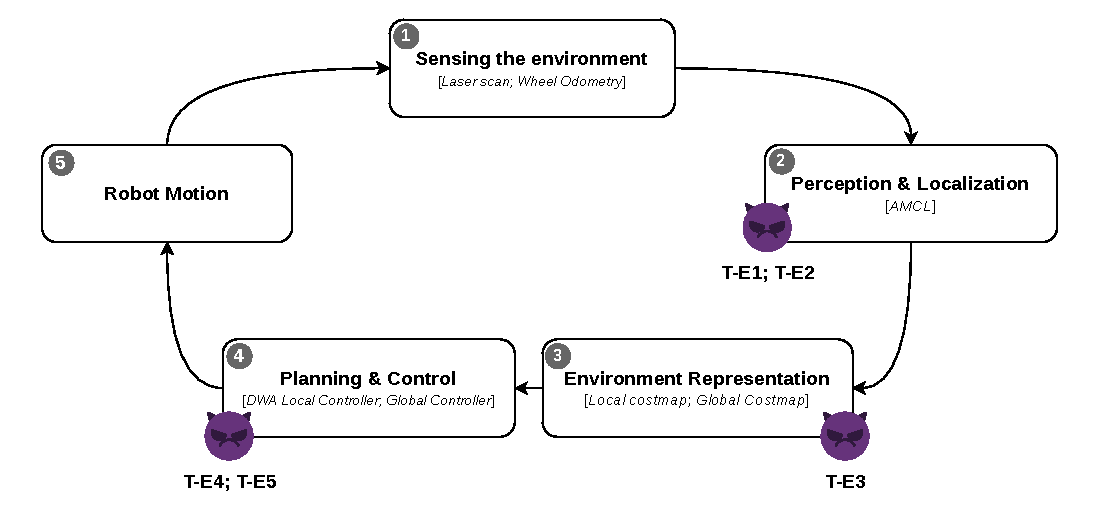
\includegraphics[width=0.9\columnwidth]
        {figures/navigation_pipeline.pdf}
    \caption{TurtleBot3 navigation pipeline and selected components in which the delay was injected for each experiment.}
    \label{fig:turtlebot-pipeline}
\end{figure}

\noindent We introduced delays at different points of the pipeline to investigate if the impact of a timing violation depends not only on its duration but also on the position of the delayed operation. In fact, the
same delay can have different consequences depending on if it affects localization output, frame synchronization, environment representation, or the control-command path. A delayed producer may continue to generate correct information in
the value domain but becomes temporally stale before reaching its consumers. Conversely, a delay in the local planner directly postpones
the generation of the next velocity command and may reduce the effective control frequency.

\noindent Unlike the ArduPilot case study, this one did not identify a single waypoint transition as a common activation phase. Instead, we associated each injected delay with a specific navigation operation. The delay was applied whenever the corresponding callback or control cycle reached the instrumented \texttt{usleep} operation during the active navigation task. In particular, the timing perturbation was repeated throughout the mission. This allowed us to observe the direct effect of each suspension and the possible cumulative effects, such as stale data, missed update periods, or longer gaps between consecutive velocity commands.

\noindent We considered the following injection points:
\begin{itemize} [nosep]
    \item \textbf{AMCL pose-publication:} Once the AMCL has processed the laser scan and computed the pose, it published the result through \texttt{pose\_pub\_.publish(...)}. We inserted a delay immediately before this operation. In particular, the sleep only postponed the publication of the result. This experiment was designed to evaluate if a correct pose becomes stale in the time domain before being consumed;
    
    \item \textbf{AMCL TF-publication:} TF transformations associate the position information and the sensor frames at specific timestamps. They are used by several downstream components. We inserted a delay immediately before \texttt{sendTransform(...)}. Delaying this operation may affect not only the delivery time of one message but also transform availability, sensor synchronization, callback execution, and consumer waiting;

    \item \textbf{Local-costmap update loop:} This component generates obstacle representation used by the local planner, integrating laser measurements and robot-pose information. Delaying the update loop increases the interval between costmap refreshments and may cause the planner to operate on an older obstacle representation;
    
    \item \textbf{Local-controller execution:} We inserted the delay in the velocity command generation path immediately
    before 
    
    \texttt{computeVelocityCommands()}. This sleep directly affects the component that generates the physical-control output. During the sleep, the robot state, odometry, sensor data, and costmap information may continue
    to evolve, while no new velocity command is computed.

\end{itemize}

\noindent \textbf{Logging and recorded measurements}

\noindent We collected experimental data at two complementary levels: source-level timing CSV files, and ROS bag recordings. These datasets describe, respectively, the internal timing effect at the instrumented code location, its propagation to the observable ROS navigation pipeline with the final outcome of each execution.
For every modified source location, we implemented a custom CSV logger. The logger records one row for each instrumented callback, update iteration, or control cycle. While the exact fields depend on the selected injection point, all configurations record the requested software delay, the delay effectively measured around \texttt{usleep()}, and the difference between the two values. The measured delay is obtained using a monotonic wall clock, because \texttt{usleep()} only guarantees that the calling thread is suspended for at least the requested interval and the actual wake-up instant can be affected by operating-system scheduling.
Moreover, in each target function, timestamp extraction and file output were placed after the operation under investigation or outside the interval used to calculate the primary timing metric. This prevents the CSV disk operation from being included in the measured execution interval. However, source-level logging still introduces timestamp-acquisition, value-formatting, and file I/O overhead. For this reason, each experiment includes a zero-delay configuration in which the complete instrumentation remains enabled but no intentional suspension is introduced. The delayed configurations are primarily compared with this matched instrumented baseline.
\\
The AMCL pose-publication logger records the timestamp of the source laser scan and the instant at which the resulting pose is published. Their difference represents the temporal displacement of the localization result: 
\begin{equation}
TD_{\text{pose}} = t_{\text{pose-publication}} - t_{\text{scan}}.
\end{equation}
The injected delay does not directly alter the numerical pose estimate already computed by AMCL, instead, it postpones its availability, potentially making the estimate stale with respect to the current robot state.
\\
The AMCL TF-publication logger records the scan timestamp, the timestamp assigned to the transform, and the instant at which \texttt{sendTransform()} is reached. These values are used to calculate both the end-to-end TF temporal displacement and the age of the transform timestamp at transmission time. This distinction is relevant because a delayed TF update may affect several consumers requiring temporally valid transformations between the map, odometry, sensor, and robot frames.

\noindent The local-costmap logger records the execution duration of 
\\
\texttt{updateMap()}, the interval between consecutive completed updates, and the age of the previous completed update immediately before the next refresh. Since the local costmap was configured at 10 Hz, its nominal update period was 100 ms. We define its update temporal displacement as: 
\begin{equation}
TD_{\text{costmap}} = T_{\text{update interval}} - 100 \text{ ms}.
\end{equation}
The previous-update age is used as a indicator for costmap staleness. In a way, it indicates how long the latest completed costmap remained available before a new refresh.
Then, as regards the local-controller experiments, there are two complementary views of the command-generation path:
\begin{itemize}
    \item The analysis in \texttt{MoveBase::executeCycle()} focuses on the latency of an individual control cycle, measuring how long the command-generation path takes from the beginning of the cycle to the publication of the resulting velocity command. It separates this end-to-end latency into the artificial waiting time before the planner invocation, the execution time of \texttt{computeVelocityCommands()}, the time required for the command to become available, and the additional latency before its publication. This decomposition makes it possible to determine if a command is published late because the planner itself requires more computation or because an otherwise stable planner is invoked later in the cycle;
    \item The experiments involving 
    
    \texttt{DWAPlannerROS::computeVelocityCommands()} instead measure the interval between consecutive controller invocations. Given the nominal controller frequency of 10 Hz, the controller-cycle temporal displacement is defined as: 
    \begin{equation}
    TD_{\text{DWA}} = T_{\text{DWA cycle}} - 100 \text{ ms}.
    \end{equation}
\end{itemize}
Hence, the two controller measurements are not treated as equivalent. Command-publication latency describes the internal latency of one control cycle, while the DWA cycle interval describes the loss of periodicity between consecutive controller executions.
In addition to the custom CSV files, we recorded a ROS bag for each run. A ROS bag is a timestamped recording of the messages exchanged on selected ROS topics, which can later be analysed offline to reconstruct the system behaviour during an execution. The common recording set includes \texttt{/cmd\_vel}, \texttt{/odom}, \texttt{/scan}, \texttt{/amcl\_pose}, \texttt{/tf}, \texttt{/tf\_static}, \texttt{/move\_base/status}, \texttt{/move\_base/result}, 

\noindent \texttt{/initialpose}, \texttt{/move\_base\_simple/goal}, and \texttt{/clock}. The bag recordings preserve the externally observable navigation behaviour and make it possible to reconstruct the mission interval, robot motion, command stream, sensor proximity, and final action outcome using the same extraction method across the different injection points.
\\
\noindent \textbf{Evaluation metrics} \\
We treated each navigation run as one independent experimental repetition. The multiple callbacks, costmap updates, and controller cycles recorded during the same run were used to characterize its internal timing behaviour. These observations belong to the same process execution and share the same scheduling conditions, robot trajectory, and experimental configuration.
We first aggregated the event-level timing observations separately for each run. Depending on the metric, we report the mean, median, standard deviation, minimum, maximum, and 95th percentile. The median represents the typical timing behaviour while reducing the influence of isolated outliers. The 95th percentile and maximum describe the tail of the timing distribution, which is relevant when evaluating real-time execution because a limited number of large delays may still disrupt the control pipeline.
\\
The requested delay is the independent experimental variable. The measured delay and delay error are used as a check to verify that the intended suspension was actually introduced.
\\
The primary internal timing metrics depend on the injection stage:
\begin{itemize}[nosep]
    \item For the localization experiments, we use pose temporal displacement, TF temporal displacement, and TF timestamp lag;
    \item For the local costmap, we use update-completion interval, update temporal displacement, and previous-update age;
    \item For the controller experiments, we use scheduling displacement, planner-computation time, command-publication latency, DWA cycle interval, and DWA cycle displacement.
\end{itemize}
These internal metrics are summarized in Table~\ref{tab:turtlebot_internal_metrics}.
We then extract a common set of \textit{end-to-end} metrics from the ROS bags, considering only the portion of each recording corresponding to the effective mission window.
This mission window begins when the \texttt{/move\_base\_simple/goal} message is recorded, indicating the real effective start of the mission, and ends when the corresponding \texttt{/move\_base/result} is received, signaling the termination and outcome of the navigation action. Mission duration is calculated only for successfully completed or explicitly terminated actions. For runs without a result, we record an observation duration from the goal timestamp to the end of the bag, without treating it as a mission-completion time.
\\
Command-output timing is evaluated through the mean, median, 95th-percentile, and maximum intervals between consecutive 
\\
\texttt{/cmd\_vel} messages. The corresponding effective command frequency is calculated as the inverse of the command interval. We also calculate the fraction of almost-zero commands to identify configurations associated with more frequent stopping or degraded control continuity.
\\
Navigation performance is evaluated using the mission duration, odometric path length, commanded linear and angular velocities, and the minimum valid laser range observed during the mission. The minimum laser range is used only as a comparative obstacle-proximity indicator.
\\
Mission-level outcomes include success, timeout, recovery activity, and observed collision. These discrete outcomes are analyzed together with the timing and trajectory metrics. Mission success alone is not considered sufficient evidence of nominal behaviour, because a run can reach a goal after substantial temporal displacement, command interruption and trajectory inefficiency.
\\
For runs showing visually irregular initial motion, we additionally analyze the first five seconds after the goal. The startup metrics include travelled distance, net displacement, path efficiency, changes in the sign of the angular command, reverse-command count, and time to first relevant motion. These values allow qualitative observations such as alternating rotations or short backward movements to be checked against the recorded command and odometry data.
%%% TODO IMPORTANTISSIMO; MANCA REFERENCE A TABELLA 6
\begin{table*}[t]
\centering
\caption{Internal timing metrics used in the TurtleBot3 experiments.}
\label{tab:turtlebot_internal_metrics}
\begin{tabular}{p{0.18\textwidth} p{0.20\textwidth}
                p{0.27\textwidth} p{0.27\textwidth}}
\hline
\textbf{Stage} &
\textbf{Metric} &
\textbf{Definition} &
\textbf{Interpretation} \\
\hline

AMCL pose-publication &
Pose temporal displacement &
Time between the source laser-scan timestamp and the publication of the resulting AMCL pose. &
Age of the localization result when it becomes available to downstream components. \\

AMCL TF-publication &
TF temporal displacement &
Time between the source scan timestamp and the transmission of the corresponding transform. &
End-to-end delay affecting the availability of localization information through the TF tree. \\

AMCL TF-publication &
TF timestamp lag &
Difference between the transform-transmission time and the timestamp assigned to the transform. &
Age of the TF information at the instant in which it is transmitted. \\

Local costmap &
Update-completion interval &
Time between the completion of two consecutive local-costmap updates. &
Actual periodicity of the costmap producer task. \\

Local costmap &
Update temporal displacement &
Update-completion interval minus the nominal 100-ms update period. &
Deviation of the costmap-update cycle from its expected timing. \\

Local costmap &
Previous-update age &
Time elapsed since the previous completed update immediately before the next refresh. &
Indicator for the time during which the last completed costmap remains the most recent available version. \\

Local controller &
Scheduling displacement &
Difference between the expected controller activation time and the observed activation time. &
Delay accumulated before the planner starts its computation. \\

Local controller &
Planner-computation time &
Execution time of \texttt{computeVelocityCommands()}. &
Computational cost of the local-planning operation, excluding the intentional pre-planner wait when measured separately. \\

Local controller &
Command-publication latency &
Time from the beginning of the control cycle, or from the selected reference point, to the publication of the resulting command. &
End-to-end internal latency before the new velocity command becomes externally observable. \\

DWA controller &
DWA cycle interval &
Time between two consecutive invocations of \texttt{computeVelocityCommands()}. &
Actual periodicity of the DWA controller task. \\

DWA controller &
DWA cycle displacement &
DWA cycle interval minus the nominal 100-ms controller period. &
Loss of controller periodicity relative to its expected 10 Hz execution rate. \\

\hline
\end{tabular}
\end{table*}

\subsubsection{Design and results of the (small-scale) case study}
\\
\leavevmode\par
\noindent We organized the TurtleBot3 case study into six experimental configurations, covering four semantically different stages of the ROS Navigation pipeline, which are: localization-result publication, TF transmission, local-costmap production, and local-control execution. Each configuration includes a zero-delay condition, except for T-E0, which represents the independent clean baseline without source-level timing instrumentation.
\\
The experiments do not all use the same delay set or the same number of independent runs. We keep each configuration and delay condition separate and report its actual number of repetitions. 
\\
The zero-delay configurations maintain the complete timing and logging code while introducing no intentional suspension. They are used as matched references for evaluating the timing and behavioural effects of the corresponding delayed configurations. T-E0 is instead used to determine if the additional measurement code substantially changes the nominal navigation behaviour.
\\
All the various configurations are summarized in Table~\ref{tab:turtlebot3_configs} and are discussed below.

\begin{table*}[t]
\centering
\caption{TurtleBot3 experimental configurations}
\label{tab:turtlebot3_configs}
% Aumenta lo spazio verticale tra le righe (di default è 1)
\renewcommand{\arraystretch}{1.5} 
\begin{tabular}{
    p{0.06\textwidth}
    p{0.40\textwidth}
    p{0.26\textwidth}
    p{0.16\textwidth}
}
\hline
\textbf{ID} &
\textbf{Target component and injection point} &
\textbf{Analyzed delay conditions} &
\textbf{Independent runs} \\
\hline

\textbf{T-E0} &
\raggedright No injection; clean ROS Navigation Stack &
No intentional delay &
5 \\

\textbf{T-E1} &
\raggedright AMCL pose delivery, immediately before \newline
\texttt{pose\_pub\_.publish()} &
0, 20, 50, 100, 200, 500, and 1000-ms &
5 per condition \\

\textbf{T-E2} &
\raggedright AMCL TF delivery, immediately before \newline
\texttt{tfb\_->sendTransform()} &
0, 20, 50, 100, and 200-ms &
5 per condition \\

\textbf{T-E3} &
\raggedright \texttt{Costmap2DROS::mapUpdateLoop()}, \newline immediately before
\texttt{updateMap()}; local costmap only &
0, 200, 500, 1000, and 2000-ms &
5 runs for 1000-ms; 3 runs for the other conditions \\

\textbf{T-E4} &
\raggedright \texttt{MoveBase::executeCycle()}, immediately before \newline
\texttt{tc\_->computeVelocityCommands(cmd\_vel)} &
0, 20, 50, 100, 200, 500, and 1000-ms &
5 per condition \\

\textbf{T-E5} &
\raggedright Beginning of \texttt{DWAPlannerROS::}\newline\texttt{computeVelocityCommands()} &
0, 200, 500, 1000, and 2000-ms &
1 run for 2000-ms; 3 runs for the other conditions \\

\hline
\end{tabular}
\end{table*}
\\
\noindent \textbf{T-E0: Clean navigation baseline}
\\
T-E0 represents the independent clean baseline of the TurtleBot3 case study. Its purpose is to characterize the nominal timing and navigation behaviour of the unmodified ROS Navigation Stack before introducing source-level delay instrumentation. This configuration also provides the reference required to determine if the instrumented 0-ms conditions of T-E1--T-E5 preserve the original system behaviour.
\\
We executed five independent runs using the common navigation scenario described in Section~\ref{sec:2.2.1}. No intentional software delay was introduced and none of the selected pose-publication, TF-publication, local-costmap, or controller injection points was modified. Still, we maintained the ROS bag recording procedure to collect the goal, action result, velocity commands, odometry, laser scans, localization estimates, and TF messages required for the external navigation analysis.
\\
In this experiment, the timing behaviour is characterized through the externally observable command stream. The median interval between consecutive \texttt{/cmd\_vel} messages was approximately 100 ms, consistently with the configured 10-Hz controller frequency.
All five runs successfully reached the assigned goal. No collision or recovery behaviour was observed. Mission duration ranged from approximately 23.10 to 23.70 s, with a median of approximately 23.30 s. The odometric path length remained between approximately 4.41 and 4.46 m, with a median of approximately 4.42 m. The minimum valid laser range was also consistent across the runs, remaining between approximately 0.256 and 0.273 m.
These results indicate that the selected scenario produced a repeatable nominal navigation behaviour. The limited variation in mission duration, travelled distance, command periodicity, and obstacle proximity makes T-E0 a suitable clean reference for the subsequent experiments. In particular, substantial differences between T-E0 and an instrumented 0-ms condition would indicate that the source-level instrumentation, rather than the intentional delay, affected the navigation behaviour. 

\noindent \textbf{T-E1: AMCL pose-publication delay}
\\
T-E1 evaluates if postponing the publication of the pose estimated by AMCL produces a measurable localization temporal displacement and if this internal timing violation propagates to command generation and mission behaviour. We inserted the controlled delay inside the AMCL laser callback, immediately before 
\\
\texttt{pose\_pub\_.publish()}. At this point, AMCL had already processed the laser observation and calculated the pose estimate, but the result had not yet been made available to the other ROS components. Hence, this experiment models a delayed localization delivery: AMCL computes the pose from the laser observation, but the result is made available to the navigation components later than expected. The pose values are not intentionally corrupted, but their usefulness may decrease because they describe an earlier robot state.
\\
We evaluated seven delay conditions: 0, 20, 50, 100, 200, 500, and 1000-ms. Each condition was repeated five times, producing 35 independent runs. The 0-ms configuration retained the complete AMCL instrumentation without introducing an intentional suspension and was used as the matched baseline for the delayed conditions.
\\
The measured sleep duration closely followed the requested delay. Across the delayed conditions, the mean measured values were approximately 20.38, 50.35, 100.34, 200.39, 500.32, and 1000.31 ms. The additional wake-up latency generally remained between approximately 0.3 and 0.4 ms. In the 0-ms condition, the approximately 0.50 ms measured interval reflects the overhead introduced by the instrumentation, since no intentional suspension was applied. The small and consistent difference between the requested and measured delays shows that the source-level modification reproduced the intended perturbation accurately.
\\
The main internal metric was the temporal displacement between the timestamp of the laser scan used by AMCL and the time at which the corresponding pose was published. In the instrumented 0-ms condition, the mean displacement across runs was approximately 25.28 ms. It increased to approximately 49.34 ms at 20-ms, 77.76 ms at 50-ms, 120.03 ms at 100-ms, 228.29 ms at 200-ms, 594.35 ms at 500-ms, and 1443.78 ms at 1000-ms. We can note that the age of the published localization estimate corresponded to the normal AMCL processing latency plus the injected delay and the remaining scheduling and publication overhead.
\\
For delays up to 200-ms, the internal displacement did not produce a systematic degradation of the externally observable command stream. The median interval between consecutive \texttt{/cmd\_vel} messages remained approximately 100 ms, and the median 95th-percentile gap remained between approximately 114 and 117 ms. The median fraction of almost-zero commands also remained close to the instrumented baseline, generally between 2.5\% and 3.4\%. 
Note that "almost zero velocity commands" refer to \texttt{/cmd\_vel} messages in which both motion components are very close to zero. Hence, a message of this type does not require either significant forward movement or significant rotation.
\\
Moreover, all five runs completed the mission in each condition from 0 to 200-ms. Median navigation duration was approximately 23.4 s in the instrumented baseline and remained between approximately 23.6 and 24.5 s across these delayed conditions. Median path length remained between approximately 4.44 and 4.50 m. Some individual runs at 20, 50, and 100-ms showed longer mission times or path lengths. However, these differences were not consistent across the delay conditions and did not increase progressively with the requested delay. The navigation stack tolerated moderate pose-publication delays in most executions of the selected scenario.
\\
A clearer external effect appeared at 500-ms. All five runs still reached the goal, but median navigation duration increased to approximately 33.7 s and median path length to approximately 4.62 m. While the median \texttt{/cmd\_vel} gap remained close to 100-ms, the 95th percentile gap increased to approximately 132 ms. This means that, in a typical run, 95\% of the intervals between consecutive commands were no longer than about 132 ms, while the remaining 5\% were longer. The median stop-command fraction also increased to approximately 26.5\%. This condition represents a degraded but still operational state, in which the controller continued to publish at its typical nominal rate but produced more interruptions and required more time to complete the navigation task.
\\
The strongest effects occurred at 1000-ms. Four of the five runs reached the goal, whereas one terminated with an ABORTED status. In the aborted run, \texttt{move\_base} reported that no valid control command could be found, even after the recovery behaviours had been executed. Among the four successful runs, navigation duration ranged from approximately 46.2 to 96.2 s, with a median of approximately 72.8 s. Their median path length was approximately 4.97 m.
The typical \texttt{/cmd\_vel} interval at 1000-ms still remained close to 100 ms, showing that the pose-publication delay did not directly reduce the nominal frequency of every controller cycle. However, the command stream became less regular. The median 95th percentile gap increased to approximately 300 ms and the median stop-command fraction increased to approximately 37.5\%. The median minimum valid laser range across the five runs decreased to approximately 0.157 m. These measurements indicate longer interruptions, more frequent stopping, and a less stable navigation response even in the runs that eventually reached the goal.
\\
T-E1 therefore demonstrates a clear propagation threshold. The injected delay first produced an almost proportional increase in localization-result age while leaving mission behaviour comparatively stable. At 500-ms, the stale pose delivery was associated with longer navigation, more stops, and larger command-gap outliers. At 1000-ms, mission completion became less reliable and one execution reached the recovery and abort path. 
\\
Unlike a direct controller suspension, the controller continued to execute while receiving increasingly stale localization information. The degradation appeared through intermittent stopping, long command gaps, and recovery activity rather than through a uniform reduction of the control-cycle frequency.

\noindent \textbf{T-E2: AMCL TF-publication delay}
\\
T-E2 evaluates if delaying the publication of the AMCL map-to-odometry transform produces a measurable TF temporal displacement and if this alteration propagates to the velocity-command stream and mission behaviour. We inserted the controlled suspension inside the AMCL laser callback, immediately before 

\noindent \texttt{tfb\_->sendTransform()}, that is, the publication of the transformation. Unlike T-E1, which delays the publication of a pose message, T-E2 affects the TF tree used by multiple navigation components to relate sensor observations, localization estimates, costmaps, and planning frames.
\\
We planned seven delay conditions: 0, 20, 50, 100, 200, 500, and 1000-ms. Complete and analyzable datasets were obtained for the conditions from 0 to 200-ms. Each of these five conditions was repeated five times, producing 25 independent runs. The 0-ms configuration maintained the complete TF instrumentation without introducing an intentional suspension and was used as the matched reference for the delayed conditions.
\\
Preliminary executions were also attempted with 500-ms and 1000-ms delays. In these attempts, the navigation task did not progress correctly from its initial phase: a valid destination could not be established reliably and the robot appeared not to react after the attempted goal assignment. We cannot determine if the behaviour resulted from the TF-publication delay, a mission-initialization problem, an unsuitable execution procedure, or another issue in the virtualized ROS and Gazebo environment. The 500-ms and 1000-ms attempts are consequently documented as unsuccessful preliminary trials and are excluded from the quantitative analysis.
\\
For the analyzed conditions, the measured sleep duration closely followed the requested delay. The mean measured values across runs were approximately 20.37, 50.41, 100.51, and 200.57 ms for the four delayed conditions. In the instrumented 0-ms condition, the measured timing interval was approximately 0.39 ms and represented instrumentation and function-call overhead. The small and consistent difference between the requested and measured delays shows that the source-level modification reproduced the intended perturbation accurately.
\\
The main internal timing metric was the temporal displacement between the timestamp of the laser scan processed by AMCL and the instant at which the corresponding transform was transmitted. The mean displacement across runs was approximately 24.64 ms in the instrumented baseline. It increased to approximately 48.89 ms at 20-ms, 79.61 ms at 50-ms, 120.27 ms at 100-ms, and 234.62 ms at 200-ms. The temporal displacement increased almost proportionally to the injected delay, while the remaining difference was related to normal AMCL processing, scheduling, and transform-transmission overhead.
\\
The logger also measured the difference between the transform-transmission time and the timestamp assigned to the transform. In the adopted AMCL configuration, the TF timestamp was positioned approximately 500 ms ahead of the source scan timestamp. Consequently, this metric was negative in the normal runs: the transform was transmitted before the future timestamp assigned to it. Its mean value changed from approximately -475.36 ms in the 0-ms condition to -451.11, -420.39, -379.73, and -265.38 ms as the delay increased. The injected suspension progressively consumed the temporal margin provided by the future-dated transform, even though the mean value remained negative even at 200-ms.
\\
Despite the clear increase in internal TF displacement, the externally observable navigation behaviour remained comparatively stable. The median interval between consecutive \texttt{/cmd\_vel} messages remained approximately 100 ms in every condition. The median 95th-percentile gap ranged from approximately 115 to 118 ms and the stop-command fraction also remained low, with condition medians between approximately 2.1\% and 3.3\%. Hence, the TF delay did not produce a systematic reduction in the controller-output frequency over the tested range.
\\
All 25 runs reached the assigned goal. Median mission duration was approximately 23.30 s in the instrumented baseline and remained between approximately 23.30 and 24.20 s across the delayed configurations. Median odometric path length remained between approximately 4.42 and 4.46 m. The minimum valid laser range varied between conditions, but no monotonic reduction was observed as the delay increased. These measurements do not indicate a systematic degradation in navigation efficiency, command continuity, or obstacle proximity up to the analyzed 200-ms delay.
\\
T-E2 therefore demonstrates that delaying TF transmission creates a measurable and increasing internal temporal displacement, but this timing alteration did not substantially propagate to the mission-level behaviour in the selected scenario. The transform continued to be transmitted with a timestamp ahead of its publication instant, and this remaining margin may have helped the navigation components tolerate the introduced delay. Moreover, the environment was static, so the geometric relationship represented by an older transform may have remained temporarily usable despite its delayed delivery.
This conclusion is limited to the five conditions for which complete recordings were available. Since the 500-ms and 1000-ms preliminary attempts did not produce analyzable datasets, we cannot determine how the system would behave when the injected suspension approached or exceeded the future-timestamp margin. In particular, those attempts cannot support the conclusion that a large TF-publication delay caused the robot to stop or prevented mission initialization.

\noindent \textbf{T-E3: Local-costmap update delay}

\noindent T-E3 evaluates if a controlled delay in the local-costmap producer task generates a measurable update temporal displacement and if this internal timing violation propagates to command generation and navigation behaviour. We inserted the delay in 

\noindent \texttt{Costmap2DROS::mapUpdateLoop()}, immediately before 
\\
\texttt{updateMap()}.
\\
We evaluated five delay conditions: 0, 200, 500, 1000, and 2000-ms. The 0-ms, 200-ms, 500-ms, and 2000-ms conditions were repeated three times. The 1000-ms condition was initially repeated three times, but two additional runs were collected after an irregular startup motion was observed in one execution. Hence, we obtained five independent runs for this condition and allowed us to examine if the behaviour was isolated or recurrent.
\\
The instrumented 0-ms condition maintained the complete local-costmap logger without introducing an intentional suspension. In the delayed conditions, the measured sleep duration closely followed the requested value. The median measured delays were approximately 200.06, 500.06, 1000.06, and 2000.06 ms. The difference between requested and measured delay therefore remained close to 0.06 ms, indicating that the injected suspension closely matched the intended value.
\\
The local costmap was configured with an update frequency of 10 Hz, corresponding to a nominal period of 100 ms. In the 0-ms condition, the median interval between completed updates was approximately 101.45 ms, with a median displacement of 1.45 ms. The interval increased to approximately 203.05, 502.80, 1003.25, and 2011.23 ms for the 200-ms, 500-ms, 1000-ms, and 2000-ms conditions, respectively. Relative to the nominal period, the corresponding median update displacements were approximately 103.05, 402.80, 903.25, and 1911.23 ms.
\\
The age of the previous completed update increased consistently with the injected delay. Its median value was approximately 92.5 ms in the 0-ms condition and increased to approximately 200.6, 500.5, 1000.4, and 2000.4 ms in the delayed configurations. These results confirm that the experiment didn't suspend the thread: it progressively increased the time for which the latest completed local costmap remained the only available update.
\\
Despite this severe internal timing alteration, the main mission-level indicators remained largely stable, with the notable exception of the temporary startup irregularities observed in two 1000-ms runs. The median interval between consecutive \texttt{/cmd\_vel} messages remained close to 100 ms in every condition, including the 1000-ms and 2000-ms delays. Median mission duration also remained close to the instrumented baseline, ranging approximately from 23.3 to 23.6 s across the delay conditions. All seventeen runs reached the assigned goal, and no collision, recovery behaviour, or timeout was observed. Path length and minimum laser range also showed no systematic degradation as the delay increased.
\\
However, the 1000 ms-condition led to inconsistent behaviour at the beginning of the navigation task. Two out of five runs showed an irregular startup motion before continuing along the regular path. In the most evident case, startup path efficiency decreased to 0.523, the angular command changed sign six times, and fifteen reverse commands were recorded during the first five seconds. A second, less evident case had an efficiency of 0.836, seven angular sign changes, and six reverse commands. The other three runs had startup efficiencies between approximately 0.929 and 0.931, one angular sign change, and no reverse commands. The additional repetitions therefore showed that the startup instability was recurrent but not deterministic.
\\
T-E3 demonstrates that a large temporal displacement in the local-costmap update task does not necessarily produce an equivalent displacement in the controller output. In the adopted static Gazebo environment, an older costmap may remain sufficiently representative of the unchanged obstacles for the local controller to continue generating commands at its nominal frequency. Hence, despite a severe internal timing alteration, the overall navigation performance was unaffected, with the only notable exception being the transient startup irregularities at the 1000-ms delay.
\\
This interpretation is specific to the selected static scenario. The previous-update age is a indicator for costmap staleness and does not measure the exact age of the costmap at every planner access. A dynamic obstacle, a different path, or execution on a physical TurtleBot3 could impose stricter freshness requirements and produce different control or safety outcomes.

\noindent \textbf{T-E4: Delay before local-planner execution}
\\
T-E4 evaluates if delaying the invocation of the local planner increases command-generation latency and if the resulting timing violation propagates to the \texttt{/cmd\_vel} stream and mission behaviour. We inserted the controlled suspension inside 

\noindent \texttt{MoveBase::executeCycle()}, immediately before the call to 

\noindent \texttt{tc\_->computeVelocityCommands(cmd\_vel)}. At this point, the current control cycle had already started, but the local planner had not yet been invoked. This placement allowed us to distinguish a planner that starts late from a planner whose internal computation becomes more expensive.
\\
We evaluated seven delay conditions: 0, 20, 50, 100, 200, 500, and 1000-ms. Each condition was repeated five times, producing 35 independent runs. The 0-ms configuration retained the complete source-level instrumentation without introducing an intentional suspension and was used as the matched reference for the delayed conditions.
\\
The measured sleep duration closely followed the requested value. The mean measured delays across runs were approximately 20.51, 50.53, 100.44, 200.36, 500.33, and 1000.32 ms. In the instrumented baseline, the measured interval was approximately 0.41 ms and represented instrumentation and function-call overhead rather than an intentional delay. The small and consistent difference between the requested and measured delays shows that the source-level modification reproduced the intended perturbation accurately.
\\
The scheduling displacement, measured from the beginning of the control cycle to the local-planner invocation, increased consistently with the injected delay. Its mean value was approximately 0.29 ms in the instrumented baseline and increased to 20.05, 49.37, 99.61, 198.26, 492.82, and 985.88 ms as the requested delay increased. The command-publication latency showed the same tendency, rising from approximately 29.73 ms in the baseline to 47.70, 78.47, 125.67, 224.06, 512.34, and 1006.90 ms in the delayed conditions.
\\
In contrast, the execution time of \texttt{computeVelocityCommands()} did not increase with the injected delay. Its mean value remained between approximately 20 and 31 ms across the configurations and was approximately 30.80 ms in the baseline, 26.39 ms at 200-ms, 20.09 ms at 500-ms, and 21.25 ms at 1000-ms. The principal timing effect was therefore not an increase in the computational cost of the DWA algorithm. The planner was invoked later, while its own execution time remained comparatively stable.
\\
Note that, all the planner invocations returned a usable valid command, including those affected by the largest delays. This result explains this partitioning between functional correctness and temporal correctness: the local planner continued to calculate valid velocity commands, but those commands became available after progressively longer intervals.
\\
The controller was configured at 10 Hz, corresponding to a nominal period of 100 ms. For the 20-ms and 50-ms conditions, the additional latency was largely absorbed: the mean interval between command publications remained close to 100 ms. 

\noindent A transition appeared at 100 ms: the mean command-publication interval increased to approximately 126.10 ms. Approximately 93.6\% of the instrumented cycles exceeded the nominal 100 ms period.
\\
At 200 ms and above, the injected suspension could no longer be absorbed by the nominal control period. The mean publication interval increased to approximately 224.45 ms at 200-ms, 512.54 ms at 500-ms, and 1007.17 ms at 1000-ms.
\\
The ROS bag measurements showed the same propagation pattern in the externally recorded \texttt{/cmd\_vel} stream. The median gap between consecutive \texttt{/cmd\_vel} messages remained approximately 100 ms for the 0-ms, 20-ms, and 50-ms conditions. It then increased to approximately 128 ms at 100-ms, 226 ms at 200-ms, 519 ms at 500-ms, and 1011 ms at 1000-ms. The agreement between the source-level measurements and the externally recorded command stream shows that the internal scheduling displacement reached the actuation interface, that is, \texttt{/cmd\_vel} stream.
\\
The mission-level effect became clearer at 500-ms. Four runs produced a \texttt{SUCCEEDED} result, with completion times between approximately 26.0 and 32.5 s and a median of approximately 27.5 s. One run did not produce a final \texttt{move\_base} result before the recording ended and remained active during an observation window of approximately 64.8 s.
At 500-ms, the median path length across the five runs increased to approximately 4.68 m, while the median stop-command fraction increased from approximately 2.4\% in the instrumented baseline to approximately 11.1\%. In the run without a final result, the stop-command fraction reached approximately 35.8\%. The controller still generated valid commands, but their reduced frequency was associated with less continuous motion and less reliable mission completion.
At 1000-ms, four runs reached the goal, with completion times between approximately 31.4 and 45.5 s and a median of approximately 36.5 s. The remaining run did not produce a final result before the end of its approximately 54.4 s observation window. Median path length increased to approximately 5.65 m, and the median stop-command fraction reached approximately 12.8\%. The run without a terminal result travelled approximately 6.05 m and produced almost-zero velocity commands for approximately 27.4\% of its recorded command samples.
\\
Finally, T-E4 identifies three operating regions. Delays of 20 and 50-ms increased within cycle command latency but were largely absorbed without changing the nominal publication period. With a 100-ms delay, the injected suspension alone became approximately equal to the nominal controller period and once planner computation and publication overhead were included, the controller could no longer preserve its configured 10-Hz output rate. Delays of 200-ms or more cause this output rate to decrease, with delays of 500-ms and 1000-ms resulting in longer paths, more stops, and potentially no final navigation result at all.

\noindent \textbf{T-E5: DWA controller delay} \\
T-E5 evaluates how a controlled suspension introduced directly into the local controller affects its execution periodicity, the publication rate of velocity commands, and the ability of the robot to complete the assigned navigation task. We inserted the delay at the beginning of \texttt{DWAPlannerROS::computeVelocityCommands()}, before the controller gained the current robot pose and generated the next velocity command. The purpose of this configuration is not only to verify that the requested delay was applied, but also to determine if the resulting controller temporal displacement propagates to \texttt{/cmd\_vel} and to the physical navigation behaviour.
\\
We evaluated five delay conditions: 0, 200, 500, 1000, and 2000-ms. The conditions from 0 to 1000-ms were repeated three times. The 2000-ms condition was executed once and is treated as an exploratory extreme case rather than a proof of repeatable behaviour. The 0-ms configuration maintained the complete source-level instrumentation without introducing an intentional suspension and was used as the matched reference for the delayed conditions.
\\
The measured sleep durations closely followed the requested values. The median measured delays were approximately 200.06, 500.06, 1000.06, and 2000.06 ms. The resulting error remained close to 0.06 ms for all the conditions, demonstrating that the intended thread suspension was achieved.
\\
The local controller was configured to run at 10 Hz, corresponding to a nominal period of 100 ms. In the instrumented 0-ms condition, the median interval between consecutive entries into 

\noindent \texttt{computeVelocityCommands()} was approximately 100.86 ms, resulting in a median displacement of 0.86 ms. The controller interval increased to approximately 248.19, 548.92, 1048.32, and 2065.73 ms for the 200-ms, 500-ms, 1000-ms, and 2000-ms conditions, respectively. Relative to the nominal controller period, the corresponding median temporal displacements were approximately 148.19, 448.92, 948.32, and 1965.73 ms.
The nominal 100 ms period represents the target interval between consecutive controller activations, rather than an additional waiting time appended after each computation. Under normal execution, the controller waits only for the part of the period left after completing its work and when the injected suspension exceeds this budget, small or no-waiting time remains. Consequently, the measured cycle interval mainly consists of the injected delay, controller processing, and scheduling overhead, rather than the injected delay plus an additional complete 100 ms period.
\\
The internal timing violation propagated directly to the velocity-command stream. The median interval between consecutive 
\\
\texttt{/cmd\_vel} messages was approximately 100 ms in the 0-ms condition and increased to approximately 246 ms at 200 ms, 542.5 ms at 500-ms, 1030.5 ms at 1000-ms, and 2039.5 ms in the exploratory 2000-ms run. The increase in the DWA cycle interval was closely reflected in the interval between consecutive \texttt{/cmd\_vel} messages, indicating that slower controller execution resulted in less frequent command updates at the navigation output. Consequently, the robot continued to receive the previously available command for longer intervals before a new velocity correction was produced.
\\
The fraction of almost-zero velocity commands also increased with the delay.
Its median value was approximately 2.9\% in the 0-ms condition, 5.0\% at 200-ms, 10.4\% at 500-ms, and 35.0\% at 1000-ms. The exploratory 2000-ms run produced a stop-command fraction of approximately 28.9\%. These values indicate that the controller generated less continuous motion as commands became less frequent.
\\
At 200-ms, all three runs reached the goal and the main navigation metrics remained close to the instrumented baseline. The controller timing was already substantially altered, but the navigation stack tolerated the reduced command rate without a clear mission-level degradation. At 500-ms, all three runs also completed the mission, but the effect became more evident: the median mission duration increased to approximately 26.09 s, the median path length increased to approximately 4.67 m, and the larger stop fraction indicated a less continuous control output. The 500-ms condition represents a degraded but still operational state. 
A more substantial transition occurred at 1000-ms. Only one of the three runs produced a SUCCEEDED result, after approximately 66.8 s. The other two runs did not produce a \texttt{/move\_base/result} during observation windows of approximately 85 and 87 s. The robot exhibited delayed motion, overshooting, corrective manoeuvres, and longer travelled paths, which ranged approximately from 5.37 to 6.40 m.
\\
The 2000-ms condition further illustrates this loss of controller availability, even if it contains only one run. The robot did not produce a navigation result during an observation period of approximately 151.8 s and travelled approximately 12.77 m. Its minimum valid laser range reached approximately 0.12 m, considerably lower than the values observed in the nominal baseline. No collision or recovery behaviour was recorded, but the robot did not complete the task and entered a severely degraded navigation state. Since this condition was executed only once, it is used as an illustrative extreme case and not as evidence that the same outcome would occur consistently.
\\
T-E5 demonstrates a direct propagation chain from the injected suspension to controller temporal displacement, reduced \texttt{/cmd\_vel} frequency, degraded motion continuity, and eventually unreliable mission completion.

\noindent \subsubsection{Comparative analysis and answers to the research questions}
\\
We now compare the configurations to determine if the instrumentation preserved nominal behaviour, if the injected delays generated internal timing violations, and under which conditions these violations propagated to the velocity-command stream and mission-level outcomes. Since some configurations were executed on different virtualized host platforms and used different numbers of independent runs, the comparison is descriptive. Each delayed condition is primarily evaluated against its corresponding instrumented 0-ms baseline, while comparisons across injection points focus on common trends.
\\
\noindent \textbf{T-Q0. Largely yes, with a cross-platform limitation.}
\\
The instrumented zero-delay configurations largely preserved the externally observable command timing and navigation behaviour of the clean T-E0 baseline. In T-E0, all five runs reached the goal without collision or recovery behaviour. Median mission duration was approximately 23.30 s, median path length was approximately 4.42 m, and the median interval between consecutive \texttt{/cmd\_vel} messages was close to the nominal 100 ms controller period.
\\
The zero-delay conditions of T-E1--T-E5 showed the same general nominal behaviour. All of their runs reached the assigned goal, and their median \texttt{/cmd\_vel} gaps remained close to 100 ms. Median mission durations were approximately between 23.3 and 25.0 s, while median path lengths remained approximately between 4.41 and 4.58 m. No zero-delay configuration showed long stops, large command gaps, recovery activity, or missing terminal results observed in some of the high-delay conditions.
\\
The internal zero-delay measurements also remained consistent with nominal operation. More in detail, the AMCL pose and TF configurations retained their normal processing displacement, while the local-costmap and DWA-controller configurations remained close to their configured 100 ms periods.
\\
These results suggest that the instrumentation did not substantially change the robot's nominal behaviour.
However, this conclusion does not provide an exact measurement of instrumentation overhead across the complete case study. The experiments were executed on two virtual machines with different host processors, and the instrumentation was not identical at every injection point. Differences of a few seconds in mission duration or a few centimetres in path length cannot therefore be attributed exclusively to the measurement code.
\\ 
Finally, T-E0 confirms that the instrumented configurations maintained the same general nominal behaviour, while each experiment-specific 0-ms condition remains the direct reference for evaluating its delayed conditions.
\\
\noindent \textbf{T-Q1. Yes.}
\\
Controlled software delays produced measurable and increasing temporal displacement or data-age effects at every targeted navigation stage. In fact, all configurations showed the same general relation: as the requested suspension increased, the relevant result, update, planner invocation, or controller cycle became progressively later relative to its nominal timing.
\\
In T-E1, the mean AMCL pose temporal displacement increased from approximately 25.28 ms in the 0-ms condition to 228.29 ms at 200-ms, 594.35 ms at 500-ms, and 1443.78 ms at 1000-ms. T-E2 showed a similar effect on TF delivery, with mean displacement increasing from approximately 24.64 ms at 0-ms to 234.62 ms at 200-ms. For T-E1, the displacement remained approximately compatible with the added suspension up to 200-ms, while the 500-ms and 1000-ms conditions produced a more pronounced increase. T-E2 instead maintained an approximately additive relation over its analyzed range.
\\
In T-E3, the median local-costmap update displacement increased from approximately 1.45 ms at 0-ms to 103.05, 402.80, 903.25, and 1911.23 ms for delays from 200 to 2000-ms. The previous-update age increased accordingly, showing that the latest completed costmap remained the most recent available version for progressively longer intervals.
\\
The controller-side experiments produced the same overall result. In T-E4, mean scheduling displacement increased from approximately 0.29 ms at 0-ms to 985.88 ms at 1000-ms, while command-publication latency increased from approximately 29.73 to 1006.90 ms. The execution time of \texttt{computeVelocityCommands()} remained between approximately 20 and 31 ms, indicating that the planner started later but did not become computationally slower. In T-E5, the median DWA-cycle displacement increased from approximately 0.86 ms at 0-ms to 148.19, 448.92, 948.32, and 1965.73 ms as the delay increased from 200 to 2000-ms.
\\
These results confirm that the explicit suspensions generated increasing internal timing violations at all investigated injection points.
\\
\noindent \textbf{T-Q2. Partially; propagation depended on both the delay magnitude and the targeted stage.}
\\
Internal timing violations did not always reach the velocity-command stream or alter mission behaviour. In T-E2, TF temporal displacement increased up to approximately 234.62 ms, but the median \texttt{cmd\_vel} gap remained close to 100 ms and all 25 runs completed the mission with durations and path lengths close to the instrumented baseline. T-E3 showed an even stronger separation: local-costmap update displacement reached approximately 1911 ms at a 2000-ms delay, while the median \texttt{cmd\_vel} gap remained close to 100 ms and all seventeen runs reached the goal. Only temporary startup irregularities were observed in two of the five 1000-ms runs.
\\
T-E1 exhibited a delay-dependent propagation threshold. Up to 200-ms, the increasing pose displacement did not systematically alter command timing or mission completion. At 500-ms, median mission duration increased to approximately 33.7 s and the stop-command fraction to approximately 26.5\%. At 1000-ms, the command stream became less regular, the median stop fraction reached approximately 37.5\%, and one of the five runs terminated with an ABORTED result after recovery behaviour. The median \texttt{/cmd\_vel} interval still remained close to 100 ms.
\\
Propagation was more direct in the controller-side experiments. In T-E4, the median \texttt{/cmd\_vel} gap remained close to 100 ms for delays up to 50-ms, but increased to approximately 128, 226, 519, and 1011 ms at delays from 100 to 1000-ms. The 500-ms and 1000-ms conditions also produced longer paths, higher stop fractions and one run per condition ended without a final navigation result.
\\
T-E5 showed the same \textit{end-to-end} relation. The median \texttt{/cmd\_vel} gap increased from approximately 100 ms in the baseline to 246, 542.5, 1030.5, and 2039.5 ms as the injected delay increased. All runs completed the mission at 200 and 500-ms, while the latter showed measurable performance degradation. At 1000-ms, only one of three runs reached the goal, while the exploratory 2000-ms run did not produce a final navigation result.
\\
Mission-level effects generally appeared only after the perturbation became sufficiently large, first as longer navigation, stopping, and trajectory inefficiency, and later as aborted or incomplete missions. Within the tested runs, this degradation affected navigation availability and performance, while no collision was observed in the available recordings.

\noindent \textbf{T-Q3. Yes, within the limits of a descriptive cross-environment comparison.}
\\
The effect of the perturbation changed substantially with the injection point, even at comparable delay levels. At 200-ms, T-E1 and T-E2 increased AMCL pose and TF displacement to approximately 228.3 and 234.6 ms, while T-E3 produced a local-costmap update displacement of approximately 103.1 ms. However, their median \texttt{/cmd\_vel} gaps remained close to 100 ms and all runs completed the mission. In contrast, the same nominal delay increased the median command gap to approximately 226 ms in T-E4 and 246 ms in T-E5.
\\
The difference became clearer at larger delays. T-E3 retained an approximately 100 ms command gap and completed every mission even at 1000 and 2000-ms, apart from temporary startup irregularities in two runs. T-E1 instead produced longer missions and more stopping at 500-ms, followed by one aborted run at 1000-ms. T-E4 and T-E5 propagated the delay more directly to \texttt{/cmd\_vel} and, at 1000-ms, they produced command gaps of approximately one second and reduced mission-completion reliability.
\\
The comparison remains descriptive because the experiments used different numbers of runs and were executed on virtual machines with different host processors. However, the repeated contrast between producer-side and controller-side injections shows that the location of a timing perturbation strongly affects its propagation and mission-level impact.
\section{Self-assessment}

\subsection{Our critiques of our exam work}

\subsection{Discussion of our learning outcomes}


\bibliographystyle{ACM-Reference-Format}
\bibliography{sample-base}

\end{document}
